\documentclass[9pt,a4paper,twocolumn]{extarticle}

\usepackage[utf8]{inputenc}
\usepackage[T1]{fontenc}
\usepackage[spanish,es-tabla]{babel}
\usepackage[margin=1.65cm,columnsep=.65cm]{geometry}
\usepackage{lmodern,microtype,amsmath,amssymb}
\usepackage{graphicx,booktabs,tabularx,array,float,xcolor,hyperref,listings}
\usepackage{enumitem}
\usepackage{ragged2e}
\graphicspath{{imgs/}}

\newcommand{\passthrough}[1]{#1}
\providecommand{\tightlist}{%
    \setlength{\itemsep}{0pt}%
    \setlength{\parskip}{0pt}%
}

\setlist{nosep,leftmargin=*}
\hypersetup{hidelinks}

\setlength{\parindent}{0pt}
\setlength{\parskip}{3pt}
\setlength{\emergencystretch}{2em}
\raggedbottom
\setlength{\textfloatsep}{9pt}
\setlength{\intextsep}{8pt}
\setlength{\floatsep}{7pt}
\renewcommand{\topfraction}{0.9}
\renewcommand{\textfraction}{0.07}

\newcolumntype{Y}{>{\RaggedRight\arraybackslash}X}
\renewcommand{\arraystretch}{1.08}

\lstset{
    basicstyle=\ttfamily\tiny,
    breaklines=true,
    breakatwhitespace=true,
    frame=single,
    columns=fullflexible,
    showstringspaces=false,
    literate={á}{{\'a}}1
}

\begin{document}

\twocolumn[

\begin{center}

{\small\bfseries
Instituto Tecnológico de Costa Rica -- Escuela de Ingeniería en Computadores
}

\vspace{2pt}

{\small
CE1110 -- Análisis de Señales Mixtas / Tarea 2
}

\vspace{4pt}

{\LARGE\bfseries
Modelado de sistemas
}

\vspace{3pt}

{\normalsize
Banco experimental de frenado tipo ABS
}

\vspace{9pt}

{\small
\textbf{Profesor:} Luis Chavarría Zamora
\qquad
\textbf{II Semestre de 2026}
}

\vspace{6pt}

{\small
David García Cruz (2024115575)
\qquad
Saddy Guzman Rojas (2023088184)
}

\vspace{2pt}

{\small
Valerin Calderón Bran (2020033313)
\qquad
Luis Castro Montenegro (2013083843)
}

\vspace{5pt}

{\small
\textbf{Fecha de entrega:} 22 de noviembre de 2026
}
\end{center}
\vspace{-4pt}\hrule\vspace{10pt}
]
\section{Resumen}\label{resumen}

Se estudió un banco didáctico de frenado de disco tipo ABS a lazo abierto. Se revisaron las respuestas al impulso y al escalón, el muestreo y una implementación no bloqueante de PID para una fase posterior. El montaje ensayado usa un motor DC miniatura alimentado por una fuente que indicaba 1 V, un disco MDF de 12 cm, un sensor KY-033, un servomotor SG90 y una ESP32. El motor se apaga antes de aplicar el freno. En los ensayos documentados en video se comparó una corrida de giro libre con una de frenado, mediante un cambio de orden de 90 a 40 grados. Cerca de 1300 RPM, el tiempo hasta bajar de 500 RPM fue 11,300 s sin freno y 1,317 s con freno. MATLAB produjo las curvas de ambas corridas y la respuesta al impulso de un modelo local. Se distingue esta última de un impulso físico aplicado al disco.

\textbf{Palabras clave:} modelado de sistemas, frenado ABS, respuesta al
escalón, PID digital, ESP32, velocidad angular.

\section{Introducción}\label{introducciuxf3n}

Los sistemas de frenado requieren comprender la relación entre la acción
aplicada al freno y la evolución de la velocidad de una rueda. Un banco
de pruebas a escala permite estudiar esta relación de forma controlada
mediante un motor de corriente directa, un disco rotatorio, un actuador
de fricción y un sensor de velocidad. El análisis de las respuestas
transitorias es un paso previo al diseño y ajuste de un controlador.

El objetivo es explicar el modelo y la instrumentación del banco,
justificar el muestreo, mostrar una estructura de PID digital sin
\texttt{delay()} y caracterizar experimentalmente el frenado a lazo
abierto. La ESP32 mide las RPM y ordena el SG90; el motor recibe
alimentación de una fuente externa. El PID es una propuesta para una
etapa posterior y no intervino en los ensayos de esta tarea.

\section{Importancia de las respuestas al impulso y al
escalón}\label{importancia-de-las-respuestas-al-impulso-y-al-escaluxf3n}

\subsection{\textquestiondown{}Por qué son importantes para modelar
sistemas?}\label{por-quuxe9-son-importantes-para-modelar-sistemas}

Según la teoría de sistemas lineales \cite{ogata2010,franklin2015}, la \textbf{respuesta al impulso} describe cómo reacciona un sistema ante
una entrada ideal concentrada en un instante. En un sistema lineal e
invariante en el tiempo (LTI), su respuesta al impulso \(h(t)\)
permite predecir la salida frente a otras entradas mediante la
convolución:

\[
y(t)=\int_{-\infty}^{\infty}h(\tau)u(t-\tau)\,d\tau.
\]

La \textbf{respuesta al escalón} muestra cómo evoluciona la salida
cuando una entrada cambia bruscamente de un nivel constante a otro.
Permite observar el comportamiento transitorio, la estabilidad y cuando
corresponda, estimar ganancia estática, constante de tiempo, tiempo de
establecimiento y sobreimpulso. En sistemas LTI, la respuesta al escalón
es la integral de la respuesta al impulso (con condiciones iniciales
nulas).

Estas respuestas son útiles porque relacionan una entrada conocida con
la dinámica de la planta y ayudan a construir o validar modelos antes de
diseñar el controlador. \textbf{La planta real de frenado puede ser no
lineal}, por lo que las relaciones LTI se usarán como aproximaciones en
un rango de operación definido.

\subsection{Ejemplo de respuesta al impulso en el banco de
frenado}\label{ejemplo-de-respuesta-al-impulso-en-el-banco-de-frenado}

Se toma como entrada la variación de torque de frenado
\(\Delta\tau_f(t)\) y como salida la variación de velocidad
angular \(\Delta\omega(t)\). Un impulso ideal de torque no es
físicamente realizable, para aproximarlo se podría aplicar una
pulsación breve y pequeña del freno alrededor de una condición
de operación y registrar cómo cambia la velocidad.

En el modelo lineal simplificado de la sección~\ref{modelo_teorico}, si la entrada es un
torque de frenado positivo, la función de transferencia es

\[
G_f(s)=\frac{\Delta\Omega(s)}{\Delta T_f(s)}=-\frac{1}{Js+b}.
\]

Su respuesta al impulso ideal es

\[
h_f(t)=-\frac{1}{J}e^{-\frac{b}{J}t}\,\mathbf{1}(t),\qquad b>0.
\]

El signo negativo significa que aumentar el torque de frenado disminuye
la velocidad. La magnitud y rapidez de recuperación dependen de \(J\) y
\(b\). Esto es una predicción del modelo, no un resultado
medido.

\subsection{Ejemplo de respuesta al escalón en el banco de
frenado}\label{ejemplo-de-respuesta-al-escaluxf3n-en-el-banco-de-frenado}

Se hace girar el disco a una velocidad inicial aproximadamente estable.
En un instante definido se incrementa la orden de frenado de un nivel a
otro y se registra \(\omega(t)\) o las RPM a intervalos regulares. La
curva esperada muestra una reducción de velocidad, la rapidez de esa
reducción depende de la inercia, el rozamiento, el torque aplicado y el
funcionamiento del motor.

Para que el experimento sea interpretable deben registrarse las
condiciones: alimentación del motor, nivel inicial y final del freno,
tiempo del cambio y velocidad medida. Una orden de posición al
servomotor no equivale necesariamente a un escalón instantáneo de
torque: existen retardo mecánico, recorrido y fricción variable.

\textbf{Comparación resumida}

\begin{center}\begingroup\setlength{\tabcolsep}{2pt}\renewcommand{\arraystretch}{1.15}\scriptsize
\begin{tabularx}{\columnwidth}{@{}YYYY@{}}
\toprule
\textbf{Prueba} & \textbf{Entrada ideal} & \textbf{Qué aporta} & \textbf{Precaución práctica}\\
\midrule
Impulso & Pulso infinitamente corto de área finita & Información dinámica; en LTI define la respuesta a otras entradas & Se aproxima con un pulso corto, nunca se realiza exactamente\\
\addlinespace[2pt]
Escalón & Cambio súbito y sostenido de la entrada & Transitorio y régimen final; facilita estimación de parámetros & El actuador y la fricción pueden distorsionar el escalón\\
\addlinespace[2pt]
\bottomrule
\end{tabularx}\endgroup\end{center}

\subsection{Identificación de la constante de tiempo mediante un escalón}
Para una aproximación de primer orden con velocidad inicial $\omega_0$ y
velocidad final $\omega_\infty$, la respuesta es
\begin{equation}
\omega(t)=\omega_\infty+(\omega_0-\omega_\infty)e^{-t/\tau}.
\end{equation}
Al cumplirse $t=\tau$, el sistema ha recorrido aproximadamente el
63,2\,\% del cambio total hacia su velocidad final. Por ello, si la
respuesta medida se aproxima a primer orden, puede estimarse $\tau$
localizando el instante en que
\begin{equation}
\omega(\tau)=\omega_0+0.632(\omega_\infty-\omega_0).
\end{equation}
Por ejemplo, con velocidades \emph{hipotéticas} de $25$ y $10$ rad/s,
respectivamente, se obtiene $\omega(\tau)=15.52$ rad/s. Este método
requiere identificar el instante de aplicación del escalón y un valor
final suficientemente estable; no debe aplicarse sin precaución si hay
saturación, parada completa o dinámica no lineal dominante.

\section{Frecuencia de muestreo
propuesta}\label{frecuencia-de-muestreo-propuesta}

La velocidad angular de la planta es una magnitud continua, mientras que
el ESP32 la estima en instantes discretos. La elección del periodo de
muestreo debe considerar la dinámica del frenado, la resolución temporal
del sensor, la cantidad de pulsos por revolución y el tiempo requerido
para ejecutar el algoritmo.

Como hipótesis para el PID futuro se propone ejecutar el control a
\(f_s=100\,\mathrm{Hz}\), es decir \(T_s=10\,\mathrm{ms}\).
Esto no significa que haya una nueva lectura física de velocidad cada
10 ms. El firmware utilizado en los ensayos imprime una fila cada
100 ms (\(10\,\mathrm{Hz}\)); estima RPM a partir del intervalo entre
flancos aceptados del KY-033. Con una marca asumida por vuelta, a
1300 RPM transcurren aproximadamente \(60/1300=0,046\,\mathrm{s}\)
entre marcas. El valor de RPM puede repetirse en varias filas.

El descenso con freno entre aproximadamente 1300 y 500 RPM duró
1,317 s y quedó representado por unas trece filas de registro.
El umbral de rechazo de pulsos de 20 ms descarta transiciones
demasiado cercanas, pero la oscilación del disco y los pulsos
rechazados limitan la exactitud. La frecuencia de control de
100 Hz sigue siendo una propuesta teórica: todavía no se implementó
ni se verificó un PID sobre este montaje. La frecuencia de ejecución
del algoritmo y la velocidad de actualización de la estimación de RPM
son magnitudes distintas.
\subsection{Justificación cuantitativa del periodo de muestreo}
El criterio de muestreo se fundamenta en que el periodo digital debe ser suficientemente pequeño frente a la dinámica dominante de la planta \cite{franklin2015}.
En el modelo de primer orden $G_f(s)=-1/(Js+b)$, la constante de tiempo
es $\tau=J/b$. Si se adoptan únicamente para el análisis los valores
\emph{hipotéticos} $J=0.002$ kg\,m$^2$ y
$b=0.010$ N\,m\,s/rad, entonces $\tau=0.2$ s. Como criterio de diseño
inicial, se requieren al menos diez actualizaciones de control por
constante de tiempo:
\begin{equation}
T_s\leq\frac{\tau}{10}=0.02\,\mathrm{s},\qquad f_s\geq50\,\mathrm{Hz}.
\end{equation}
Se propone $f_s=100$ Hz, es decir, $T_s=10$ ms, equivalente a veinte
actualizaciones durante la $\tau$ \emph{hipotética}. Esta selección
debe revisarse con la dinámica real y el tiempo de ejecución del
controlador antes de poner el PID en servicio.
La frecuencia de actualización del PID no equivale necesariamente a la
resolución de la medición: a 200 RPM, un encoder de 20 pulsos por vuelta
produce $200(20)/60=66.67$ pulsos/s, o solamente $0.667$ pulsos en
10 ms en promedio. En ese caso conviene medir tiempos entre flancos o
usar una ventana de estimación más larga, sin bloquear el lazo de control.

\section{Implementación digital del controlador
PID}\label{implementaciuxf3n-digital-del-controlador-pid}

El controlador previsto utiliza el error \(e[k]=r[k]-\omega[k]\), donde
\(r[k]\) es la referencia de velocidad y \(\omega[k]\) la velocidad
medida. Una formulación discreta preliminar, basada en la discretización de un PID continuo \cite{ogata2010}, es:

\[
I[k]=I[k-1]+e[k]T_s,\qquad
D[k]=\frac{e[k]-e[k-1]}{T_s},
\]
\[
 u[k]=K_p e[k]+K_i I[k]+K_d D[k].
\]

La orden debe limitarse al intervalo físico admisible del actuador y
contemplar protección contra saturación integral (\emph{anti-windup}).
En un freno que solo puede aumentar o disminuir fricción, el sentido de
la acción y el signo del error deberán comprobarse experimentalmente.

No se debe utilizar \passthrough{\lstinline!delay()!} para marcar el
periodo de control porque bloquea la ejecución y puede retrasar la
adquisición del sensor, la comunicación y otras tareas. Se propone una
temporización no bloqueante con \passthrough{\lstinline!micros()!} \cite{arduinoMicros} y un
intervalo de ejecución fijo.


\subsection{Ejemplo de implementación no bloqueante en ESP32}
El siguiente listado es una \emph{plantilla de control} para los pines
y componentes reales, no el firmware usado para las mediciones.
Incluye lectura del periodo entre pulsos del KY-033 y orden al SG90.
Las ganancias se dejan en cero para evitar presentarlas como
ajustadas; antes de activar un PID deben obtenerse y validarse.
Se incluye limitación de salida y protección elemental contra
saturación integral. La captura experimental se hizo a lazo abierto
con órdenes manuales.
\begin{lstlisting}[language=C++,basicstyle=\ttfamily\tiny,breaklines=true,frame=single]
#include <Arduino.h>
#include <ESP32Servo.h>
Servo freno;
const int PIN_SENSOR = 34, PIN_SERVO = 18;
const uint32_t TS_US = 10000; // 100 Hz
uint32_t proximo = 0;
float kp = 0.0f, ki = 0.0f, kd = 0.0f;
float integral = 0.0f, errorPrevio = 0.0f;
float referencia = 0.0f; // rad/s
volatile uint32_t pulsoPrevio = 0, periodoUs = 0;
volatile uint32_t ultimoPulso = 0;

void IRAM_ATTR detectarMarca() {
  uint32_t ahora = micros();
  if (ultimoPulso && ahora - ultimoPulso <= 20000) return;
  if (pulsoPrevio) periodoUs = ahora - pulsoPrevio;
  pulsoPrevio = ultimoPulso = ahora;
}
float leerVelocidad() { // Una marca por vuelta
  noInterrupts();
  uint32_t p = periodoUs, ultimo = ultimoPulso;
  interrupts();
  if (!p || micros() - ultimo > 1000000) return 0.0f;
  return 2.0f * PI * 1000000.0f / p; // rad/s
}
void aplicarFreno(float u) {
  freno.write((int)(90.0f - 50.0f*u)); // 90 a 40 grados
}
void setup() {
  Serial.begin(115200);
  pinMode(PIN_SENSOR, INPUT);
  freno.attach(PIN_SERVO);
  freno.write(90);
  attachInterrupt(digitalPinToInterrupt(PIN_SENSOR),
                  detectarMarca, FALLING);
  proximo = micros() + TS_US;
}
void loop() {
  uint32_t ahora = micros();
  if ((int32_t)(ahora - proximo) >= 0) {
    proximo += TS_US;
    const float Ts = TS_US * 1e-6f;
    float velocidad = leerVelocidad();
    // Para un freno: error positivo si
    // la velocidad supera la referencia.
    float error = velocidad - referencia;
    float derivada = (error-errorPrevio)/Ts;
    float candidato = integral + error*Ts;
    float sinLimite = kp*error + ki*candidato
                     + kd*derivada;
    float u = constrain(sinLimite,0.0f,1.0f);
    if (u == sinLimite) integral = candidato;
    aplicarFreno(u);
    errorPrevio = error;
    Serial.printf("%.3f,%.3f,%.3f\n",
                  velocidad, referencia, u);
  }
}
\end{lstlisting}
El uso de \texttt{micros()} permite ejecutar el cálculo al alcanzar
cada instante de muestreo sin detener el procesador con
\texttt{delay()}. Debe verificarse que el cálculo y las comunicaciones
terminen dentro de $T_s$; también deben incorporarse medidas de
seguridad, gestión de sobretiempos y un cálculo de derivada menos
sensible al ruido. El signo del error se ha escogido para que una
velocidad excesiva incremente el frenado; se validará con el actuador.

\section{Arquitectura y diagrama de
bloques}\label{arquitectura-y-diagrama-de-bloques}

\subsection{Descripción general}\label{descripciuxf3n-general}

El sistema es un banco didáctico de frenado de una rueda o disco. Un
motor de corriente directa (CD) proporciona el movimiento rotacional
inicial. Durante la prueba, un mecanismo aplica fricción sobre el disco
para reducir su velocidad angular. Un sensor mide la velocidad y entrega
una señal que puede ser adquirida por un microcontrolador.

En la versión completa del proyecto, el microcontrolador ejecutará un
controlador PID digital y modificará la acción del freno según el error
entre la velocidad de referencia y la velocidad medida. Para la
construcción solicitada en el punto 6 de esta tarea, se ensambla la
planta con sus componentes, pero sin implementar todavía el
controlador. Por tanto, las pruebas de esta etapa se realizan a lazo
abierto, con una acción de frenado establecida manualmente o mediante
una orden de prueba.

\subsection{Diagrama de bloques}\label{diagrama-de-bloques}

La figura~\ref{fig:arquitectura} muestra cómo va a quedar la arquitectura completa del sistema al final del proyecto. Sin embargo, para las pruebas en lazo abierto de esta etapa, dejamos el controlador PID deshabilitado y mandamos la señal de frenado de forma directa e independiente. 

\begin{figure}[H]
    \centering
    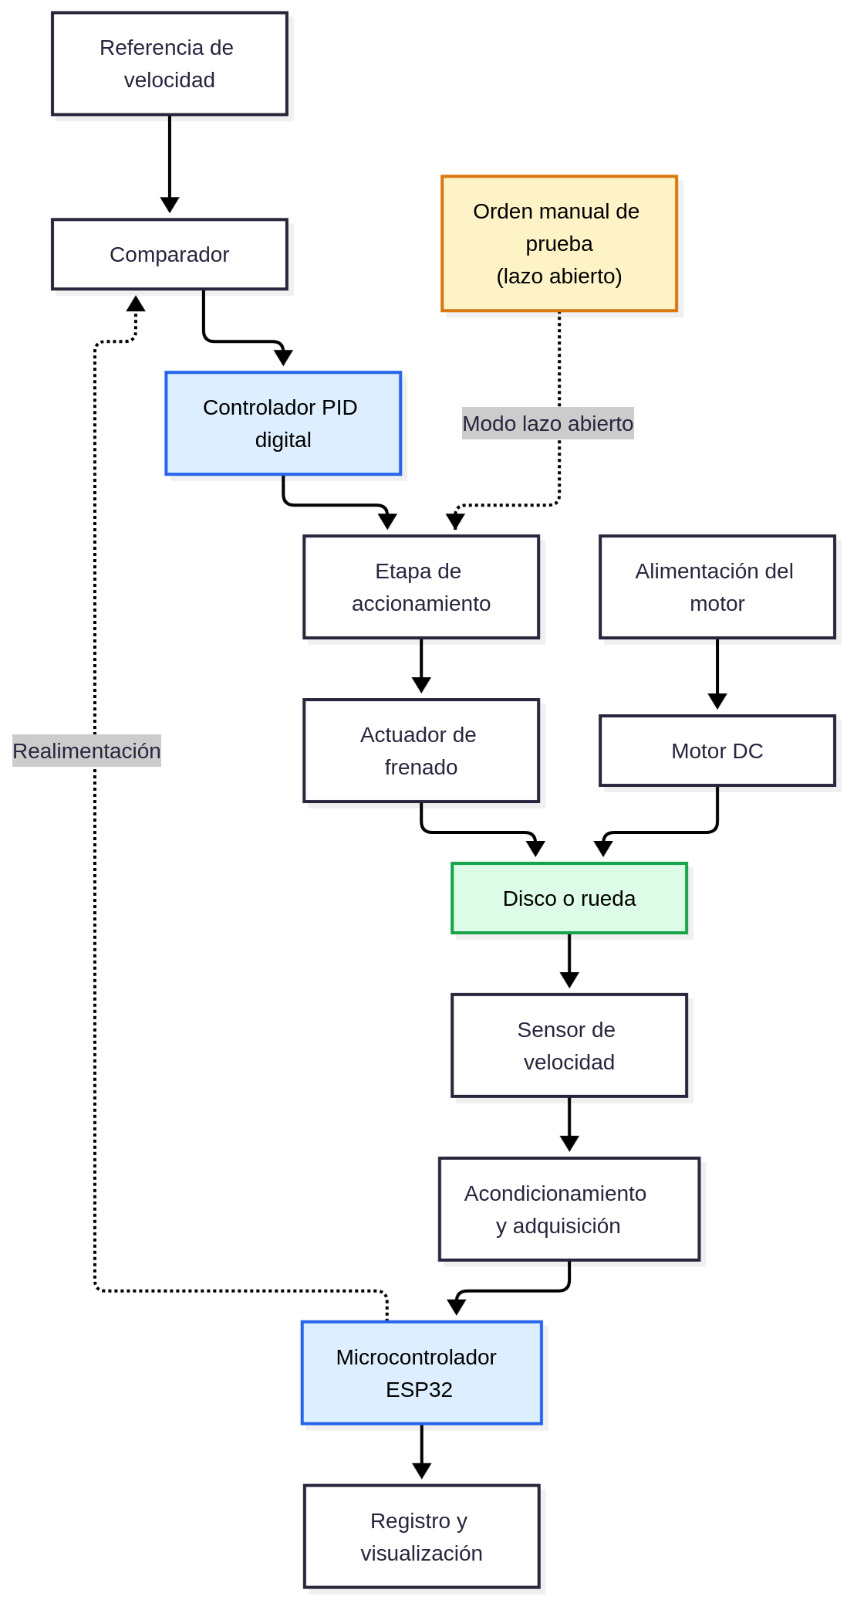
\includegraphics[width=0.94\columnwidth,height=0.43\textheight,keepaspectratio]{diagrama_sistema.jpeg}
    \caption{Arquitectura funcional propuesta.}
    \label{fig:arquitectura}
\end{figure}


Aunque el esquema incluye tanto el lazo cerrado definitivo como esta ruta alternativa de prueba, en esta entrega todavía no usamos la realimentación del sensor para ajustar el freno automáticamente.



\subsection{Interpretación de la arquitectura de control}
El ESP32 se encarga de correr el comparador, el algoritmo PID y toda la lógica de adquisición de datos. Por su parte, la planta física continua abarca el motor, el disco y el mecanismo de fricción, mientras que el sensor convierte el giro en pulsos eléctricos que luego procesamos digitalmente para calcular la velocidad. Cuando trabajamos en lazo cerrado, el error entre la referencia y la velocidad medida entra al PID, y su salida mueve el servomotor del freno. En cambio, durante la prueba a lazo abierto dejamos prefijada la orden del freno y solo registramos lo que mide el sensor, sin que eso modifique la acción de frenado de forma automática. Dentro del esquema funcional, el PID va integrado en el procesamiento digital del microcontrolador y la alimentación del motor se maneja por aparte de la señal que le mandamos al freno.

\subsection{Descripción de los componentes}

\begin{center}\begingroup\setlength{\tabcolsep}{2pt}\renewcommand{\arraystretch}{1.15}\scriptsize
\begin{tabularx}{\columnwidth}{@{}YYY@{}}
\toprule
\textbf{Componente} & \textbf{Tipo / dominio} & \textbf{Función}\\
\midrule
Motor de corriente directa & Continuo, eléctrico y mecánico & Entrega el par para acelerar el disco antes de cada ensayo. Su alimentación debe poder reducirse o desconectarse de manera controlada.\\
\addlinespace[2pt]
Disco o rueda & Continuo, mecánico rotacional & Elemento que gira y sobre el cual actúa el freno. Debe estar firmemente sujeto al eje.\\
\addlinespace[2pt]
Mecanismo de freno y zapata & Continuo, mecánico & Produce fricción sobre el disco. La intensidad de frenado depende de la presión o fuerza aplicada.\\
\addlinespace[2pt]
Servomotor u otro actuador & Interfaz eléctrica discreta y salida mecánica & Convierte una orden eléctrica en movimiento para presionar o liberar el freno. \\
\addlinespace[2pt]
Sensor de velocidad & Interfaz física y señal eléctrica & Detecta el giro del disco. \\
\addlinespace[2pt]
Acondicionamiento de señal & Analógico y/o digital, según el sensor & Adapta la salida del sensor para que pueda ser leída correctamente.\\
\addlinespace[2pt]
Microcontrolador & Discreto/digital & Adquiere las mediciones, calcula la velocidad angular y registra los datos. En el sistema final también ejecutará el PID digital.\\
\addlinespace[2pt]
Referencia y comparador & Discreto/digital & La referencia define la velocidad deseada y el comparador calcula el error entre referencia y velocidad medida. Se utiliza en el sistema completo.\\
\addlinespace[2pt]
Controlador PID & Discreto/digital & Calcula la acción de control a partir del error. Debe considerar los límites físicos del freno y evitar la acumulación excesiva del término integral. \\
\addlinespace[2pt]
Registro y visualización & Discreto/digital & Guarda o muestra tiempo, velocidad medida, referencia y acción de frenado para analizar los ensayos.\\
\addlinespace[2pt]
Fuente de alimentación & Eléctrico & Suministra energía al motor, microcontrolador, sensor y actuador según sus especificaciones.\\
\addlinespace[2pt]
\bottomrule
\end{tabularx}\endgroup\end{center}

\subsection{Elementos continuos}\label{elementos-continuos}

Los procesos físicos evolucionan continuamente en el tiempo. En este
banco destacan:

\begin{itemize}
\tightlist
\item
  La corriente y el par desarrollados por el motor.
\item
  La posición y velocidad angular del disco.
\item
  La fricción entre la zapata y el disco.
\item
  La desaceleración provocada por el frenado.
\end{itemize}

La variable física principal que se desea observar es la velocidad
angular del disco, representada por \(\omega(t)\).

\subsection{Elementos discretos}\label{elementos-discretos}

Los elementos discretos procesan o transmiten información mediante
señales muestreadas o estados digitales:

\begin{itemize}
\tightlist
\item
  Lectura del sensor por el microcontrolador.
\item
  Cálculo de RPM o velocidad angular a partir de pulsos o mediciones.
\item
  Generación de órdenes para el actuador.
\item
  Cálculo del error y del PID en la versión completa.
\item
  Almacenamiento y visualización de datos.
\end{itemize}

El microcontrolador trabaja con muestras separadas por un periodo de
muestreo \(T_s\). Así, representa el comportamiento continuo mediante
valores discretos.

\subsection{Señales principales}\label{seuxf1ales-principales}

\begin{center}\begingroup\setlength{\tabcolsep}{2pt}\renewcommand{\arraystretch}{1.15}\scriptsize
\begin{tabularx}{\columnwidth}{@{}YYY@{}}
\toprule
\textbf{Señal} & \textbf{Símbolo} & \textbf{Descripción}\\
\midrule
Orden de frenado & $u(t)$ o $u[k]$ & Acción aplicada al mecanismo. En la prueba a lazo abierto se define manualmente o mediante una secuencia de prueba.\\
\addlinespace[2pt]
Velocidad angular & $\omega(t)$ & Velocidad física instantánea del disco.\\
\addlinespace[2pt]
Velocidad medida & $\omega[k]$ & Estimación discreta obtenida mediante el sensor y el microcontrolador.\\
\addlinespace[2pt]
Referencia & $r[k]$ & Velocidad deseada en el sistema completo con PID.\\
\addlinespace[2pt]
Error & $e[k]$ & Diferencia entre referencia y velocidad medida: $e[k]=r[k]-\omega[k]$.\\
\addlinespace[2pt]
Periodo de muestreo & $T_s$ & Tiempo entre adquisiciones consecutivas.\\
\addlinespace[2pt]
\bottomrule
\end{tabularx}\endgroup\end{center}

\begin{center}\rule{0.5\linewidth}{0.5pt}\end{center}

\section{Representación matemática y respuesta esperada de la
planta}\label{modelo_teorico}

\subsection{Variables y supuestos}

Se propone un modelo preliminar de dinámica rotacional para la
rueda/disco y el freno. Se supone eje rígido, momento de inercia
equivalente constante y rozamiento viscoso aproximado. Se desprecia
inicialmente la flexibilidad mecánica, el juego y la dependencia de la
fricción con temperatura y velocidad. Estos supuestos deberán revisarse
al construir el banco.

\begin{center}\begingroup\setlength{\tabcolsep}{2pt}\renewcommand{\arraystretch}{1.15}\scriptsize
\begin{tabularx}{\columnwidth}{@{}YYY@{}}
\toprule
\textbf{Símbolo} & \textbf{Significado} & \textbf{Unidad}\\
\midrule
$J$ & Inercia equivalente del rotor y disco & kg·m²\\
\addlinespace[2pt]
$\omega(t)$ & Velocidad angular & rad/s\\
\addlinespace[2pt]
$\tau_m(t)$ & Torque motor & N·m\\
\addlinespace[2pt]
$\tau_f(t)$ & Torque de frenado (opuesto al giro) & N·m\\
\addlinespace[2pt]
$b$ & Coeficiente de fricción viscosa equivalente & N·m·s/rad\\
\addlinespace[2pt]
$u_f(t)$ & Orden eléctrica/digital al actuador & Según implementación\\
\addlinespace[2pt]
\bottomrule
\end{tabularx}\endgroup\end{center}

Aplicando la segunda ley de Newton para rotación, como aproximación mecánica de primer orden \cite{ogata2010}:

\[
J\frac{d\omega(t)}{dt}=\tau_m(t)-b\omega(t)-\tau_f(t).
\tag{1}
\]

Ya en el banco real, el torque del motor y el del freno no siempre actúan por separado ni son fáciles de aislar, pero esta ecuación nos funcionó como base para empezar a plantear el modelo.

\subsection{Función de transferencia mecánica
simplificada}
Para ver variaciones pequeñas cerca de un punto de operación, dejamos $\tau_m$ fijo y tratamos el torque de frenado como si fuera una entrada limpia. Restando el equilibrio y aplicando Laplace con condiciones iniciales en cero para las desviaciones:

\begin{equation}
\begin{aligned}
(Js+b)\Delta\Omega(s)&=-\Delta T_f(s),\\
G_f(s)&=\frac{\Delta\Omega(s)}{\Delta T_f(s)}
=-\frac{1}{Js+b}.
\end{aligned}
\end{equation}

Vale aclarar que esta función de transferencia conecta el torque de frenado con la velocidad angular y no directamente el ángulo del servo con las RPM. Para representar la entrada real del banco se tienen que incluir o identificar cómo se traduce la orden $u_f$ en el torque $\tau_f$, ya que en esa etapa suelen aparecer no linealidades y saturación.

En cambio, si se deja el freno quieto y se toma el torque del motor como entrada, la relación mecánica queda como $\Delta\Omega(s)/\Delta T_m(s)=1/(Js+b)$. 

\subsection{Derivación de la función de transferencia}
Se linealiza alrededor de un punto de operación, siguiendo el enfoque clásico de modelado por variables de desviación \cite{franklin2015}.
El balance de torques para el disco es
\begin{equation}
J\dot\omega(t)=\tau_m(t)-b\omega(t)-\tau_f(t).
\end{equation}
Se estudian variaciones pequeñas alrededor de un equilibrio
$(\omega_0,\tau_{m0},\tau_{f0})$ que cumple
$0=\tau_{m0}-b\omega_0-\tau_{f0}$. Restando esta igualdad del
balance dinámico y suponiendo $\Delta\tau_m(t)=0$, se obtiene
\begin{equation}
J\frac{d\Delta\omega(t)}{dt}+b\Delta\omega(t)
=-\Delta\tau_f(t).
\end{equation}
Aplicando Laplace con condiciones iniciales nulas para las variaciones:
\begin{equation}
(Js+b)\Delta\Omega(s)=-\Delta T_f(s).
\end{equation}
Por tanto,
\begin{equation}
\boxed{G_f(s)=\frac{\Delta\Omega(s)}{\Delta T_f(s)}
=-\frac{1}{Js+b}.}
\end{equation}
Para un incremento de torque de frenado constante $\Delta\tau_f>0$,
la respuesta teórica es
\begin{equation}
\omega(t)=\omega_0-\frac{\Delta\tau_f}{b}
\left(1-e^{-bt/J}\right),\quad t\geq0.
\end{equation}
Con los valores \emph{hipotéticos} $J=0.002$ kg\,m$^2$,
$b=0.010$ N\,m\,s/rad, $\omega_0=25$ rad/s y
$\Delta\tau_f=0.15$ N\,m, resulta
\begin{equation}
\boxed{\omega(t)=25-15(1-e^{-5t})\ \mathrm{rad/s}.}
\end{equation}
Se predicen $\tau=0.20$ s, velocidad final $10$ rad/s y tiempo de
establecimiento aproximado $4\tau=0.80$ s. Estos resultados no son
mediciones de la planta. Si el incremento de frenado supera el torque
que permite un equilibrio con $\omega\geq0$, la predicción lineal
podría arrojar velocidades negativas; físicamente la rueda se detiene
y el modelo debe incorporar la restricción $\omega\geq0$ y la fricción
estática. La relación entre el comando del servo y el torque real
requiere identificación experimental.

\subsection{Respuesta teórica al escalón de frenado}

Si el disco gira inicialmente a \(\omega_0\), el torque del motor se
mantiene constante y se aplica un incremento ideal constante
\(\Delta\tau_f>0\) en \(t=0\), el modelo (1) predice:

\[
\boxed{\omega(t)=\omega_0-\frac{\Delta\tau_f}{b}\left(1-e^{-t/\tau}\right)},
\qquad \tau=\frac{J}{b},\quad b>0.
\tag{3}
\]

Aquí \(\omega_0\) representa la velocidad de equilibrio previa al
cambio. Para el modelo lineal, el cambio final de velocidad sería

\[
\Delta\omega_{\infty}=-\frac{\Delta\tau_f}{b},
\qquad K_f=-\frac{1}{b},
\qquad \tau=\frac{J}{b}.
\]

El modelo de primer orden no presenta sobreimpulso y se
aproxima exponencialmente a un nuevo equilibrio, el tiempo de
establecimiento al 2 \% es aproximadamente \(4\tau\). Si el frenado
detiene físicamente el disco, la expresión deja de ser válida al llegar
a \(\omega=0\), porque el sistema real no puede continuar con velocidad
negativa bajo el mismo supuesto de frenado unidireccional. Si \(b\) es
despreciable, la aproximación pasa a una desaceleración casi lineal:
\(\omega(t)\approx\omega_0-(\Delta\tau_f/J)t\), hasta detenerse.
La figura~\ref{fig:escalon_teorico} ilustra esa respuesta teórica
con parámetros hipotéticos.

\begin{figure}[H]
\centering
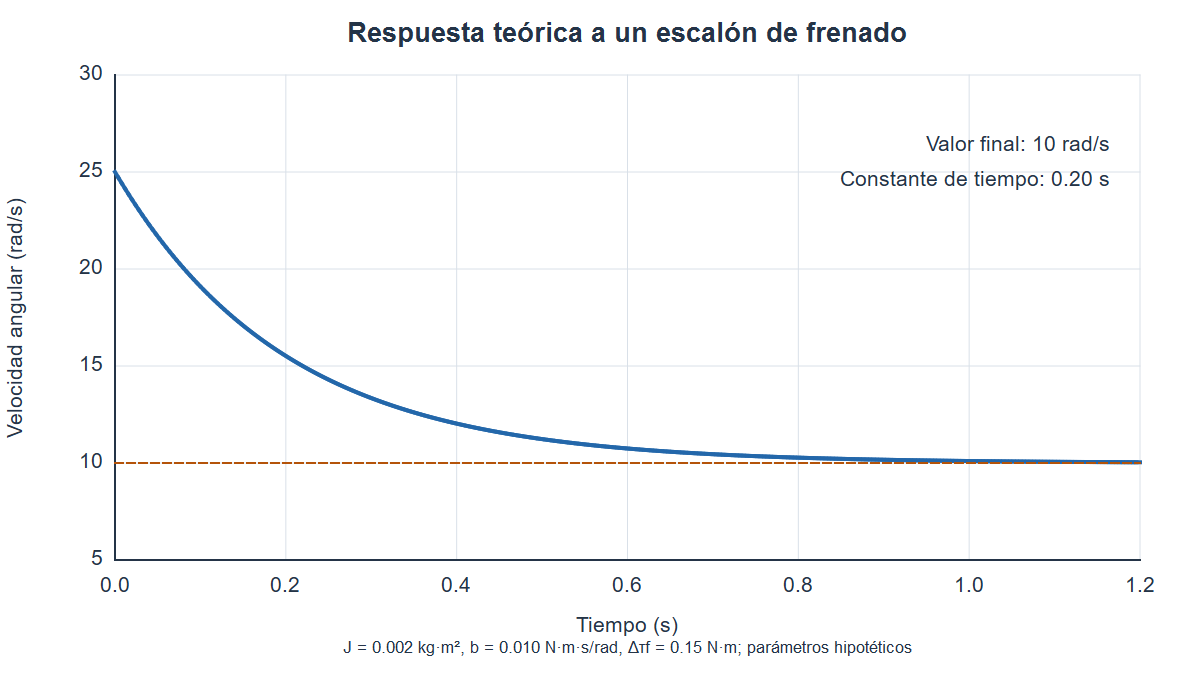
\includegraphics[width=\columnwidth]{simulacion_escalon_frenado.png}
\caption{Respuesta al escalón simulada con parámetros hipotéticos; no corresponde a una medición experimental.}
\label{fig:escalon_teorico}
\end{figure}



\subsection{Valores teóricos que se pueden
estimar}

\begin{center}\begingroup\setlength{\tabcolsep}{2pt}\renewcommand{\arraystretch}{1.15}\scriptsize
\begin{tabularx}{\columnwidth}{@{}YYY@{}}
\toprule
\textbf{Magnitud} & \textbf{Relación o método teórico} & \textbf{Estado}\\
\midrule
Velocidad angular & $\omega=2\pi\,\mathrm{RPM}/60$ & RPM registradas en los CSV de ensayo\\
\addlinespace[2pt]
Inercia de un disco macizo homogéneo & $J_d=\tfrac12 mr^2$ & Radio del MDF: 0,06 m; masa e inercia de rotor/acople no medidas\\
\addlinespace[2pt]
Constante de tiempo & $\tau=J/b$ & Requiere estimación de $J$ y $b$\\
\addlinespace[2pt]
Ganancia estática torque de freno $\rightarrow$ velocidad & $K_f=-1/b$ & Solo válida para el modelo lineal con $b>0$\\
\addlinespace[2pt]
Tiempo de establecimiento aproximado (2 \%) & $t_s\approx4\tau$ & Solo para respuesta de primer orden sin saturación\\
\addlinespace[2pt]
Desaceleración angular & $\alpha=(\tau_m-b\omega-\tau_f)/J$ & Requiere torques y parámetros\\
\addlinespace[2pt]
Tiempo de parada con desaceleración constante $a>0$ & $t_{parada}\approx\omega_0/a$ & Aproximación para un intervalo sin cambio de signo\\
\addlinespace[2pt]
\bottomrule
\end{tabularx}\endgroup\end{center}

\textbf{Alcance de los parámetros:} se conocen el radio del disco y las
RPM estimadas por el sensor. No se midieron masa, corriente, torque
del motor ni fuerza de contacto. Por ello no se presentan valores
experimentales de $J$, $b$ o torque de frenado por separado.

\subsection{Respuesta final esperada de la planta sin
controlador}

A lazo abierto, el freno recibe una orden predefinida, sin
corregirla con el error de velocidad. Si se incrementa el frenado, se
espera que las RPM disminuyan. Si el torque neto permite un nuevo
equilibrio, la velocidad tenderá a un valor menor, si el freno domina al
motor, el disco puede detenerse. Sin realimentación, el sistema
no garantiza seguir una trayectoria de velocidad ni compensar
perturbaciones automáticamente.

La forma exacta de la curva va a depender del actuador, de la fricción que haya en el montaje y de si dejamos el motor alimentado o no durante la prueba. Por eso vamos a contrastar lo que midamos en el banco con lo que predice el modelo y anotar bien las diferencias.

\subsection{Criterios de validación con el montaje real}
\label{procedimiento-de-validaciuxf3n-cuando-exista-hardware}

\begin{enumerate}
\def\labelenumi{\arabic{enumi}.}
\tightlist
\item
  Distinguir los datos conocidos (radio 0,06 m, fuente indicando 1 V,
  orden de servo y RPM estimadas) de masa, torque y alimentación exacta
  en terminales que no se midieron.
\item
  Registrar condiciones de cada corrida y conservar las marcas de
  apagado del motor y de orden del servo.
\item
  Comparar las referencias libres con las frenadas a velocidades
  iniciales parecidas.
\item
  Graficar \(\omega(t)\) en MATLAB y estimar un modelo local solo en el
  intervalo previo a la detención, con calidad de ajuste revisada.
\item
  Si la respuesta es no lineal, presenta parada o saturación,
  documentarlo en vez de forzar el ajuste de primer orden.
\item
  Dejar explícita la diferencia entre parámetros \textbf{calculados},
  \textbf{supuestos} y \textbf{medidos}.
\end{enumerate}

\section{Construcción de la planta a lazo abierto --- punto extra}

\subsection{Montaje real ensayado}

Se ensambló un banco de frenado por contacto sobre un disco MDF de
12 cm de diámetro y 3 mm de espesor. El disco gira mediante un motor
DC miniatura cuyo modelo exacto no se pudo identificar; el equipo no
dispone de su hoja de datos. Durante las corridas,
la fuente externa del motor se ajustó o indicaba 1 V. Ese valor no es
una medición con multímetro en sus terminales bajo carga.

La ESP32 registra el sensor reflectivo KY-033 en GPIO34 y envía
órdenes al servomotor SG90 por GPIO18. El SG90 y el KY-033 reciben
alimentación de la placa ESP32; no se documentaron la tensión exacta
ni la corriente de esas conexiones. La computadora recibe las
muestras y los eventos por puerto serial. El motor está conectado
directamente a la fuente externa: el módulo Mini L298N AD70178 está
disponible, pero no se instaló en estas pruebas.

El brazo del SG90 lleva un hule unido a una esponja. La esponja hace
contacto con la \textbf{cara superior} del disco, no con el borde.
La posición ordenada de 90 grados mantiene separado el freno; para
las corridas principales se envió un cambio directo a 40 grados.
Estos valores son órdenes al servo: no se midieron su posición real,
la fuerza normal ni el torque de frenado.

\begin{center}\begingroup\footnotesize\setlength{\tabcolsep}{3pt}
\begin{tabularx}{\columnwidth}{@{}p{0.28\columnwidth}Y@{}}
\toprule
\textbf{Elemento} & \textbf{Configuración del ensayo}\\
\midrule
Motor y fuente & DC miniatura de modelo no identificado; fuente externa indicando 1 V; apagado desde la fuente con cables conectados.\\
Disco y acople & MDF, diámetro 12 cm, espesor 3 mm; acople provisional con oscilación visible.\\
Sensor & KY-033 reflectivo en GPIO34; una marca por vuelta es el supuesto de la conversión a RPM.\\
Actuador & SG90 en GPIO18; hule y esponja sobre la cara superior del MDF; órdenes de 90 y 40 grados.\\
Procesamiento & ESP32 y captura serial; filas cada 100 ms y rechazo de flancos separados por 20 ms o menos.\\
\bottomrule
\end{tabularx}\endgroup\end{center}

\subsection{Conexión eléctrica y limitaciones}

El motor recibió alimentación directa de la fuente externa,
sin conexión eléctrica con la ESP32 ni con el puente H disponible.
El KY-033 entregó su señal a GPIO34 y recibió alimentación de la
placa ESP32; el SG90 recibió la orden por GPIO18 y también fue
alimentado desde esa placa. La computadora se comunicó con la
ESP32 por USB. Las fotografías muestran la conexión externa del
motor y la disposición del banco, pero no permiten identificar
con certeza los pines concretos de alimentación del servo y del
sensor. El esquema eléctrico
preliminar de diseño se excluye porque muestra un puente H y una
fuente independiente para el servo que no se utilizaron.

El acople provisional provoca oscilación del disco, especialmente
visible a velocidades bajas. El sensor rechazó múltiples flancos
durante las capturas; por ello se interpretan las RPM como
estimaciones, sin atribuir una precisión física no comprobada.
Tampoco se midieron masa del disco, momento de inercia, corriente
ni torque del motor. Estas limitaciones no impiden comparar las
curvas libres y frenadas obtenidas bajo el mismo montaje.

El funcionamiento físico y la disposición del banco se documentan
en las fotografías de la figura~\ref{fig:fotos_montaje} y en los
videos citados en la sección de evidencias.

\section{Prueba de funcionamiento a lazo abierto}
\label{prueba-de-funcionamiento-a-lazo-abierto}

En cada ensayo se aceleró el disco con la fuente del motor indicando
1 V y con el SG90 ordenado a 90 grados. Después se apagó la fuente
sin retirar los cables y se marcó manualmente el evento
\texttt{MOTOR\_OFF\_MANUAL}. En las referencias libres se mantuvo
el servo en 90 grados hasta la detención. En las pruebas de frenado
se envió posteriormente \texttt{g40}, un cambio directo de orden
de 90 a 40 grados; el evento \texttt{SERVO\_CMD} registra cuándo
se envió la orden, no el instante físico exacto de contacto.

El sensor KY-033 entregó pulsos que la ESP32 convirtió a RPM. El
capturador guardó \texttt{tiempo\_ms}, \texttt{rpm} y
\texttt{servo\_cmd\_grados} en un CSV, y las marcas de apagado y
comando en otro. El reloj se inició al obtener la primera RPM
calculable. La marca de apagado tiene incertidumbre por el tiempo de
reacción de la persona; la indicación de cero llega después de un
intervalo sin pulsos y no identifica el instante mecánico exacto
de parada.

Para el análisis mostrado en video se seleccionaron los pares
\texttt{datos\_1.csv}/\texttt{eventos\_1.csv} (giro libre) y
\texttt{datos\_2.csv}/\texttt{eventos\_2.csv} (frenado). Hay
otras capturas locales de calibración y de pruebas anteriores;
no se mezclan en las cifras presentadas aquí.
El control PID no intervino: la orden de freno fue elegida
manualmente y no se calculó a partir del error de velocidad.

\section{Evidencia audiovisual}\label{evidencias-requeridas}

El \href{https://youtu.be/hc-JIA8kH4Y}{video de la planta completa}
documenta el montaje y su funcionamiento a lazo abierto. El
\href{https://youtu.be/BWD1uK7m35k}{video de caracterización}
presenta los ensayos de giro libre y frenado y el análisis en MATLAB
de los pares 1 y 2. Son dos enlaces de evidencia para los puntos
extra 6 y 7, respectivamente. Las fotografías del montaje se
presentan en la figura~\ref{fig:fotos_montaje}.


\section{Seguridad del montaje}\label{seguridad-del-montaje}

\begin{itemize}
\tightlist
\item
  Sujetar firmemente el disco al eje y el motor a la base.
\item
  Mantener manos, cabello, ropa y cables alejados de las partes móviles.
\item
  Incorporar una protección física alrededor del disco cuando sea
  posible.
\item
  Limitar la velocidad a un nivel seguro.
\item
  Disponer de una forma accesible de desconectar la alimentación del
  motor.
\item
  Verificar que la zapata y el actuador no puedan desprenderse durante
  el giro.
\item
  Desenergizar el sistema antes de ajustar el montaje o modificar
  conexiones.
\end{itemize}

\section{Alcance del montaje}

El banco permitió iniciar el giro, estimar y registrar RPM, aplicar
una orden definida al freno y comparar su efecto con el giro libre
tras apagar el motor. Estos resultados corresponden a lazo abierto:
no demuestran todavía un sistema ABS con regulación automática ni
un PID ajustado. La oscilación del disco y el acople provisional
son limitaciones del prototipo usado para las mediciones.

\begin{center}\rule{0.5\linewidth}{0.5pt}\end{center}

\section{Caracterización experimental de la planta --- punto extra}
\label{caracterizaciuxf3n-experimental-de-la-planta-punto-extra}

El cambio de 90 a 40 grados ordenado al SG90 constituye la entrada
de escalón del ensayo. La salida observada es la velocidad del disco
estimada por el KY-033. En este protocolo el motor se apaga
\emph{antes} de aplicar el freno; el apagado y la orden del servo son
dos eventos distintos. El efecto adicional del freno se interpreta
comparando la desaceleración con corridas libres a RPM iniciales
similares. Ninguna de las dos condiciones termina en un equilibrio
positivo: ambas llegan a cero. Por ello no se estima una ganancia
estática a partir de velocidades finales.

El análisis del video utiliza los pares 1 y 2 en
\texttt{proyecto2/tarea2/capturas/}. El script
\texttt{matlab/ejecutar\_analisis.m} llama al analizador de cada
ensayo y compara la corrida libre con la frenada. Para un
\emph{modelo local} antes de bajar de 500 RPM, se aproxima la
velocidad $r(t)$ expresada en RPM mediante
\begin{equation}
\begin{aligned}
\dot r(t)&=-kr(t)-c\,u(t),\\
u(t)&=\begin{cases}
0,&\text{giro libre},\\
1,&\text{orden de freno aplicada}.
\end{cases}
\end{aligned}
\end{equation}
Aquí $k$ representa la caída libre efectiva y $c$ la desaceleración
adicional asociada a la orden de freno. No son medidas directas de
inercia ni torque. Para \texttt{tf} e \texttt{impulse} se convierte
la salida a $\omega=2\pi r/60$ en rad/s:
$G(s)=-(2\pi c/60)/(s+k)$ para la entrada normalizada $u$.
Esta función describe únicamente el intervalo ajustado. La curva
\texttt{impulse(G)} generada en MATLAB es una respuesta
\emph{del modelo}, no un impulso aplicado físicamente al disco.

El analizador de MATLAB aportado por otro integrante se adaptó
para leer los pares reales y sus eventos de apagado y frenado.
El ejemplo anterior, con motor alimentado continuamente y régimen
final, sigue como ilustración teórica; sus parámetros simulados
no corresponden a estas capturas.

\section{Resultados y discusión}\label{resultados-y-discusiuxf3n}

\subsection{Predicción teórica y alcance}

El balance de torques predice una disminución de velocidad al aumentar
el torque de freno. La figura~\ref{fig:escalon_teorico} usa parámetros
hipotéticos y un torque de motor constante; \textbf{no es la curva
medida en el prototipo}. En los ensayos reales se apagó la fuente
del motor y después se ordenó el cambio del SG90. La comparación
experimental relevante es entre giro libre y giro frenado con
velocidades similares al comienzo del tramo analizado.

\subsection{Resultados de los CSV reales}

Para la corrida libre se tomó como referencia la primera muestra
posterior al apagado entre 1250 y 1350 RPM. Para las frenadas se usó
la mediana de las cinco muestras inmediatamente anteriores a
\texttt{g40}. El tiempo de cada fila siguiente es relativo a esa
referencia, que corresponde a aproximadamente 1300 RPM; en las
frenadas coincide con el instante de la orden al servo.

\begin{center}\begingroup\footnotesize\setlength{\tabcolsep}{4pt}
\begin{tabular}{@{}lrrr@{}}
\toprule
\textbf{Corrida} & \textbf{RPM ref.} &
\(\boldsymbol{t_{<500}}\) \textbf{(s)} &
\(\boldsymbol{t_{0}}\) \textbf{(s)}\\
\midrule
Libre 1 & 1343,51 & 11,300 & 19,800\\
Freno 2 & 1368,18 & 1,317 & 2,717\\
\bottomrule
\end{tabular}\endgroup\end{center}

Los identificadores 1 y 2 corresponden a los archivos numerados
utilizados en el video. La marca manual de apagado de la fuente
precede la orden \texttt{g40} por 2,769 s en la corrida frenada.
El indicador
\(t_0\) es la primera fila con RPM iguales a cero, no el instante
exacto de parada física: el firmware espera un intervalo sin
pulsos antes de mostrar cero.

En el tramo desde cerca de 1300 hasta menos de 500 RPM, la
corrida frenada tardó 1,317 s y la libre 11,300 s: una relación
de aproximadamente 8,58 a 1. Es una comparación de \emph{dos}
ensayos con velocidades iniciales próximas, no una estimación
estadística de repetibilidad. La figura~\ref{fig:comparacion_real}
muestra ambas curvas sin filtrado adicional. No se infiere de la
relación un torque medido ni una ganancia estática.



La figura~\ref{fig:escalon_real} representa la entrada ordenada al
servo como un escalón de 90 a 40 grados y la RPM medida. La velocidad
ya venía bajando porque la fuente se apagó antes del comando; el
instante real de contacto de la esponja no se midió.



\subsection{Ajuste local y respuesta al impulso de MATLAB}

MATLAB estimó $k=0{,}0866216\;\mathrm{s}^{-1}$ en la caída libre
y $c=587{,}669\;\mathrm{RPM/s}$ como desaceleración adicional
efectiva para $u=1$. En rad/s, la transferencia local es
\begin{equation}
G(s)=\frac{-61{,}5406}{s+0{,}0866216}.
\end{equation}
El ajuste de la frenada hasta antes de 500 RPM obtuvo
$R^2=0{,}973$. La figura~\ref{fig:ajuste_local} compara las muestras
usadas con la predicción. Con una sola corrida por condición,
los parámetros no tienen incertidumbre estimada mediante repeticiones.



Se ejecutó \texttt{impulse(G)} con Control System Toolbox. La
figura~\ref{fig:impulse_matlab} inicia en un valor negativo y
\emph{asciende hacia cero}; por eso su pendiente visual es positiva.
El signo negativo expresa la reducción de velocidad ante una
entrada de frenado positiva. No es una medición de la trayectoria
física después de un impulso ni representa la detención a cero RPM.



\subsection{Incertidumbre y alcance}

La fuente indicaba 1 V, pero no se midió tensión en terminales bajo
carga. El apagado se marcó manualmente. Las RPM dependen de la
detección óptica de pulsos y el disco osciló por su acople
provisional; se observaron pulsos rechazados por el filtro de
20 ms. La ESP32 registró filas cada 100 ms, de modo que los
tiempos de cruce de un umbral tienen una resolución aproximada
de una décima de segundo además de los retrasos de detección.
El instante real de contacto de la esponja no fue medido.

El modelo ajustado describe solo la región de RPM usada; la fricción,
el retardo del servo, la cuantización de pulsos y la saturación en
cero impiden extrapolarlo a toda la maniobra. Las cifras de la tabla
proceden de los CSV reales y no de la simulación teórica.

\section{Conclusiones y recomendaciones}

El banco a lazo abierto permitió comparar una corrida libre con una
frenada bajo condiciones iniciales próximas. El cambio ordenado de
90 a 40 grados en el SG90 se asoció con una disminución del tiempo
hasta menos de 500 RPM, desde 11,300 s en giro libre hasta 1,317 s
con freno. La comparación se limita al montaje y al rango
observados; el motor ya estaba sin alimentación cuando se aplicó
el freno y ambos tipos de ensayo terminaron en cero. Una sola
corrida por condición no permite afirmar repetibilidad estadística.

El modelo de torque de primer orden aporta una explicación teórica,
pero sus parámetros físicos no se identifican por separado con
estas mediciones. La frecuencia de control de 100 Hz y el código
PID del informe son propuestas para una fase posterior; la
captura experimental utilizada imprime cada 100 ms. Las figuras de
MATLAB, las fotografías y los enlaces de video aportan las
evidencias de los puntos extra; la respuesta impulsiva mostrada
es la del modelo local, no una entrada física aplicada al disco.

\begin{thebibliography}{9}
\bibitem{ogata2010} K. Ogata, \emph{Modern Control Engineering}, 5.\textsuperscript{a} ed. Upper Saddle River, NJ: Prentice Hall, 2010.
\bibitem{franklin2015} G. F. Franklin, J. D. Powell y A. Emami-Naeini, \emph{Feedback Control of Dynamic Systems}, 7.\textsuperscript{a} ed. Boston, MA: Pearson, 2015.
\bibitem{arduinoMicros} Arduino, ``micros(),'' \emph{Arduino Language Reference}. [En línea]. Disponible: \url{https://docs.arduino.cc/language-reference/en/functions/time/micros/}. [Consultado: 18 nov. 2026].
\end{thebibliography}

\onecolumn
\section{Anexos}
\subsection{Datos y videos de evidencia}
\textbf{Datos analizados:} pares \texttt{datos\_1.csv}/
\texttt{eventos\_1.csv} y \texttt{datos\_2.csv}/
\texttt{eventos\_2.csv}; se conservaron localmente fuera de Git.
El firmware de adquisición, \texttt{matlab/ejecutar\_analisis.m}
y las cuatro gráficas reproducidas en este informe están en el
repositorio. \textbf{Videos de evidencia:}
\url{https://youtu.be/hc-JIA8kH4Y} (planta completa) y
\url{https://youtu.be/BWD1uK7m35k} (caracterización y MATLAB).
Los valores numéricos y las figuras corresponden a los pares 1 y 2;
las fotografías muestran el banco montado durante las pruebas.

\subsection{Firmware utilizado en los ensayos}
El siguiente programa es el que adquiere los pulsos del KY-033,
ordena el SG90 y emite las mediciones y los eventos seriales
utilizados para generar los CSV. Opera a lazo abierto: el PID
mostrado en la sección~\ref{implementaciuxf3n-digital-del-controlador-pid} es una propuesta y no se ejecutó durante
estas capturas. El motor recibió alimentación directa de la fuente
externa y no está controlado por la ESP32.

\lstinputlisting[language=C++,basicstyle=\ttfamily\footnotesize,breaklines=true,frame=single]{../../firmware/freno abs/src/main.cpp}


\subsection{Figuras y fotografías}
Las fotografías y las gráficas experimentales se citan en las secciones correspondientes del informe.

\begin{figure}[H]
\centering
\begin{minipage}[t]{0.47\textwidth}
\centering
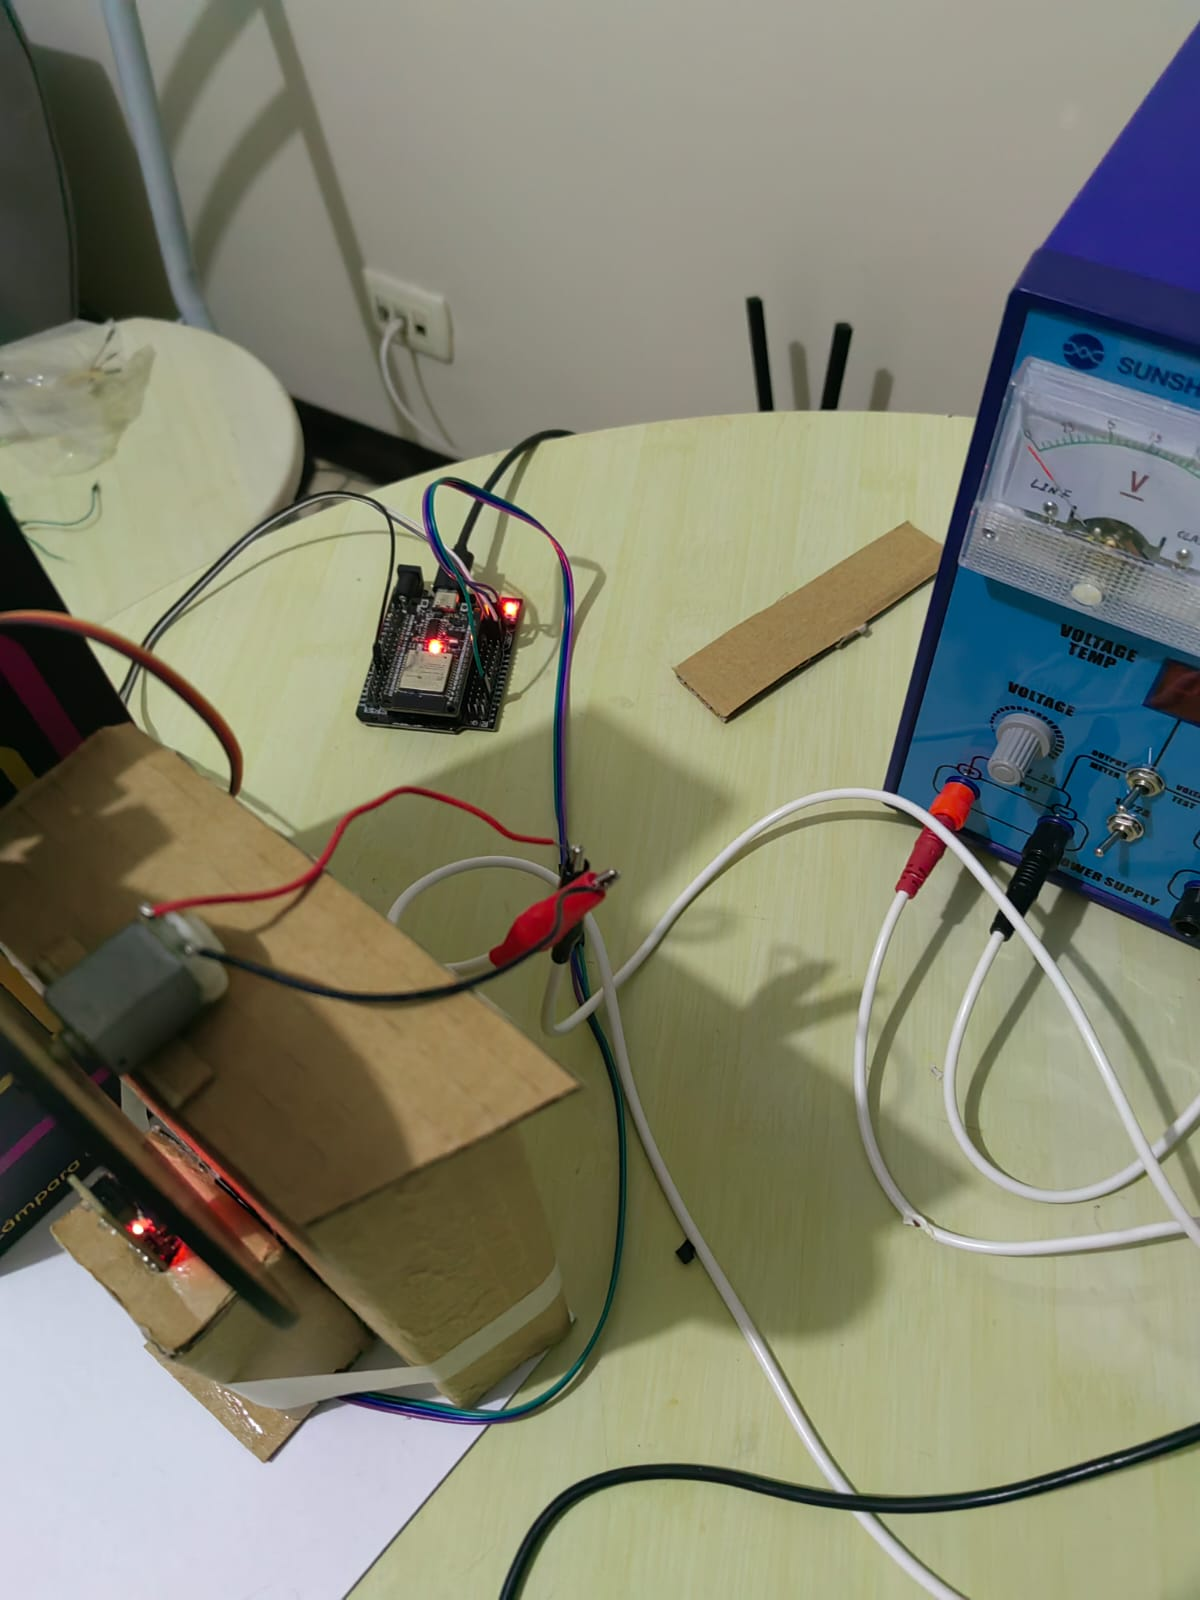
\includegraphics[width=\linewidth,height=0.32\textheight,keepaspectratio]{foto_motor_fuente.jpeg}\\
\footnotesize (a) Motor conectado a la fuente externa y ESP32 de adquisición.
\end{minipage}\hfill
\begin{minipage}[t]{0.47\textwidth}
\centering
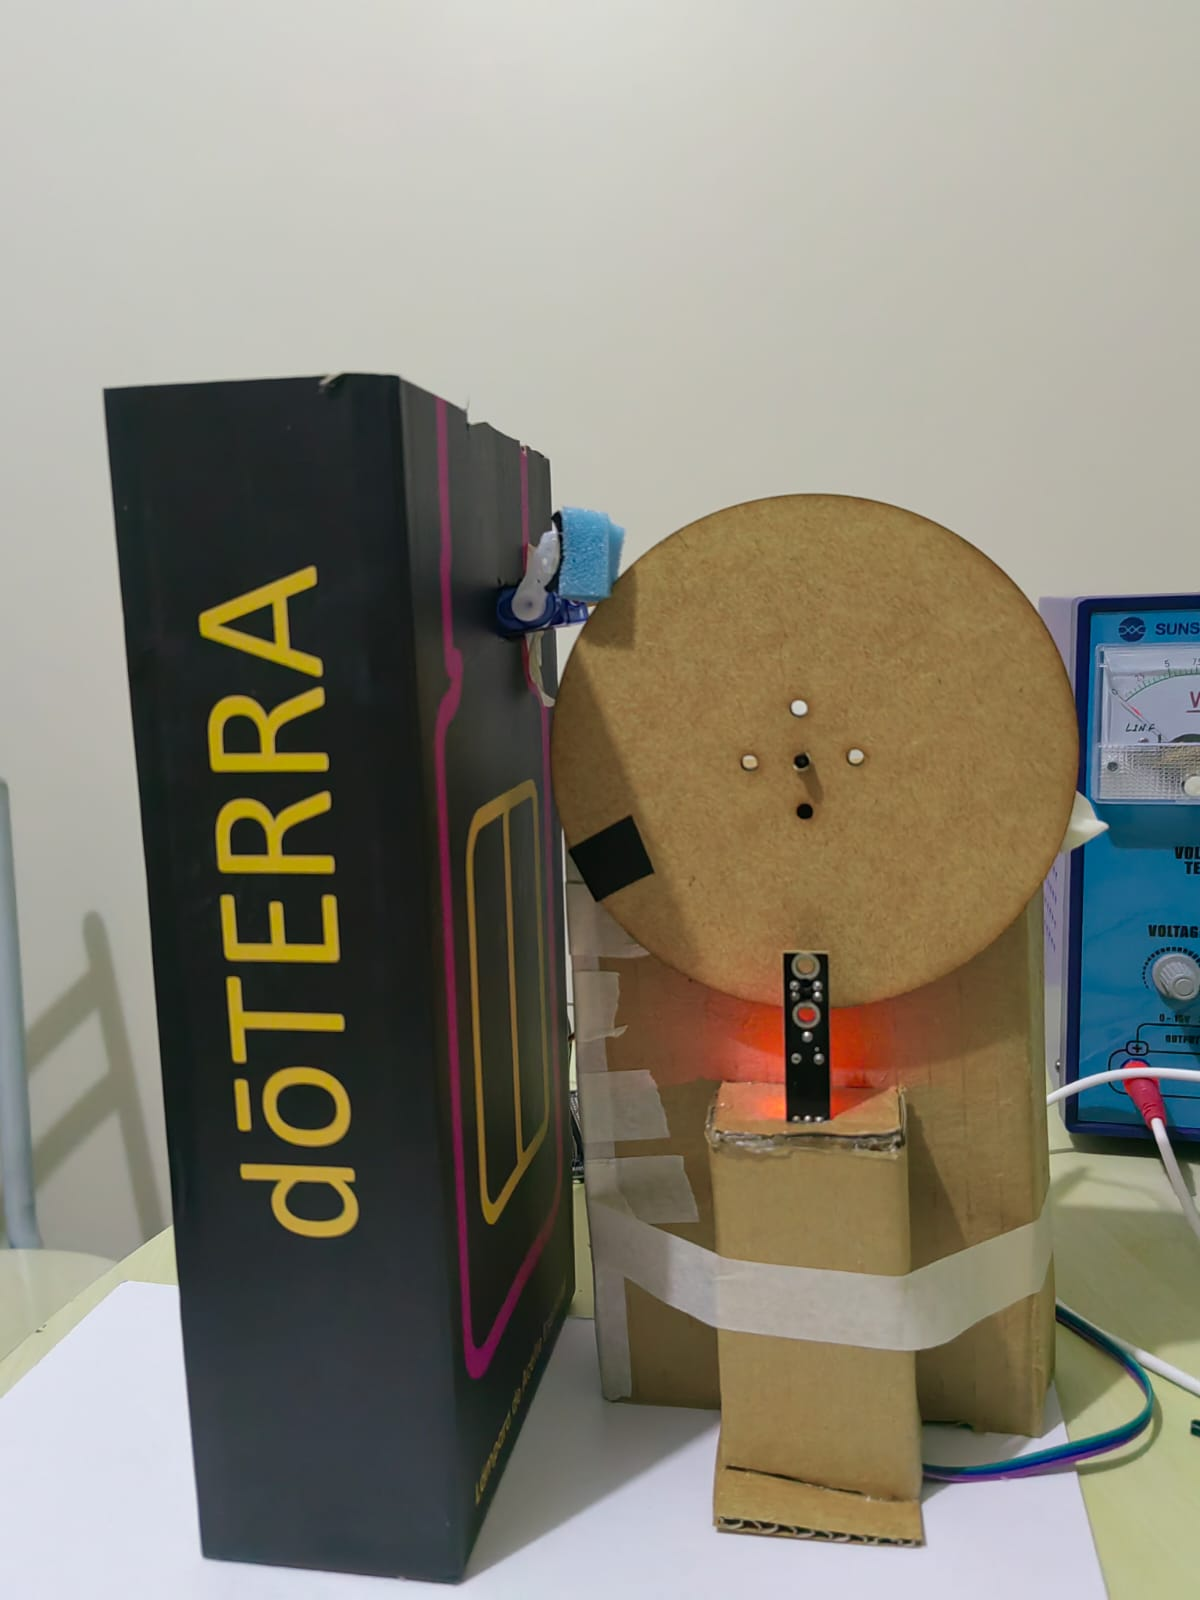
\includegraphics[width=\linewidth,height=0.32\textheight,keepaspectratio]{foto_disco_frenado.jpeg}\\
\footnotesize (b) Disco, esponja del SG90 y sensor frente a la marca.
\end{minipage}

\vspace{7pt}
\begin{minipage}[t]{0.47\textwidth}
\centering
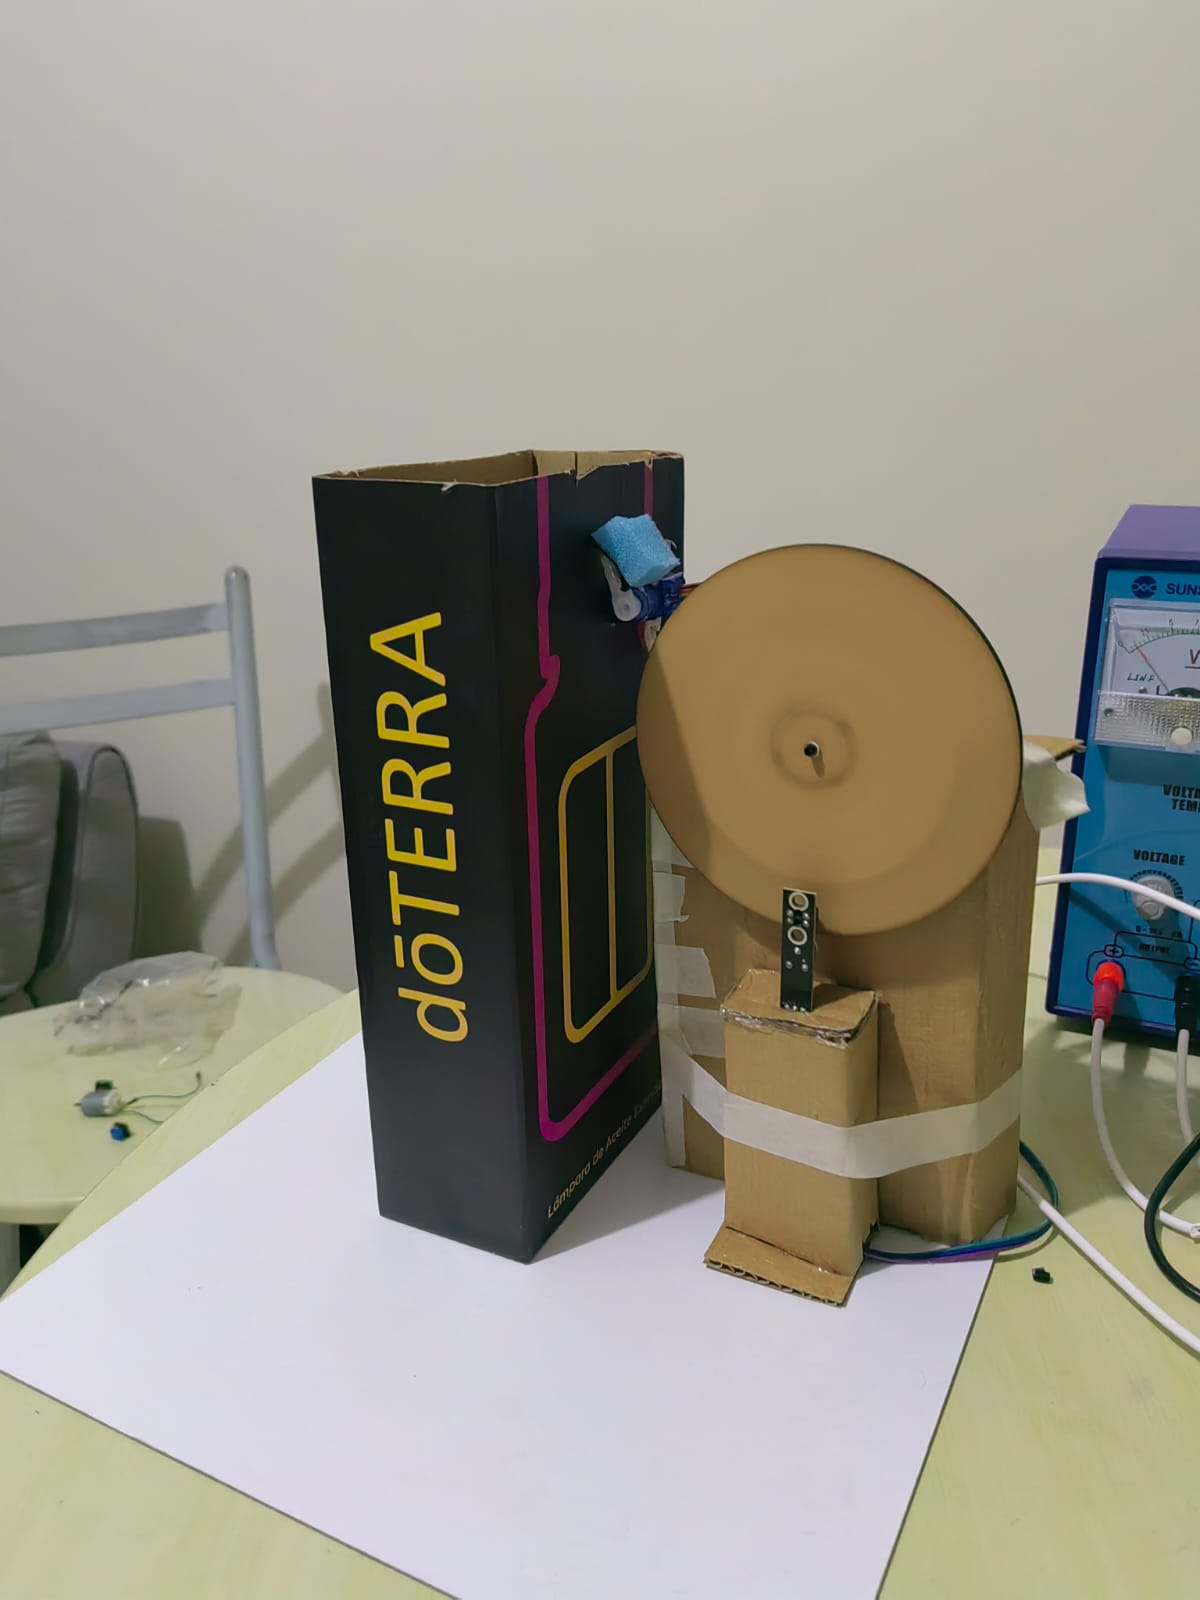
\includegraphics[width=\linewidth,height=0.32\textheight,keepaspectratio]{foto_disco_girando.jpeg}\\
\footnotesize (c) Disco en movimiento, visible por el desenfoque de la imagen.
\end{minipage}\hfill
\begin{minipage}[t]{0.47\textwidth}
\centering
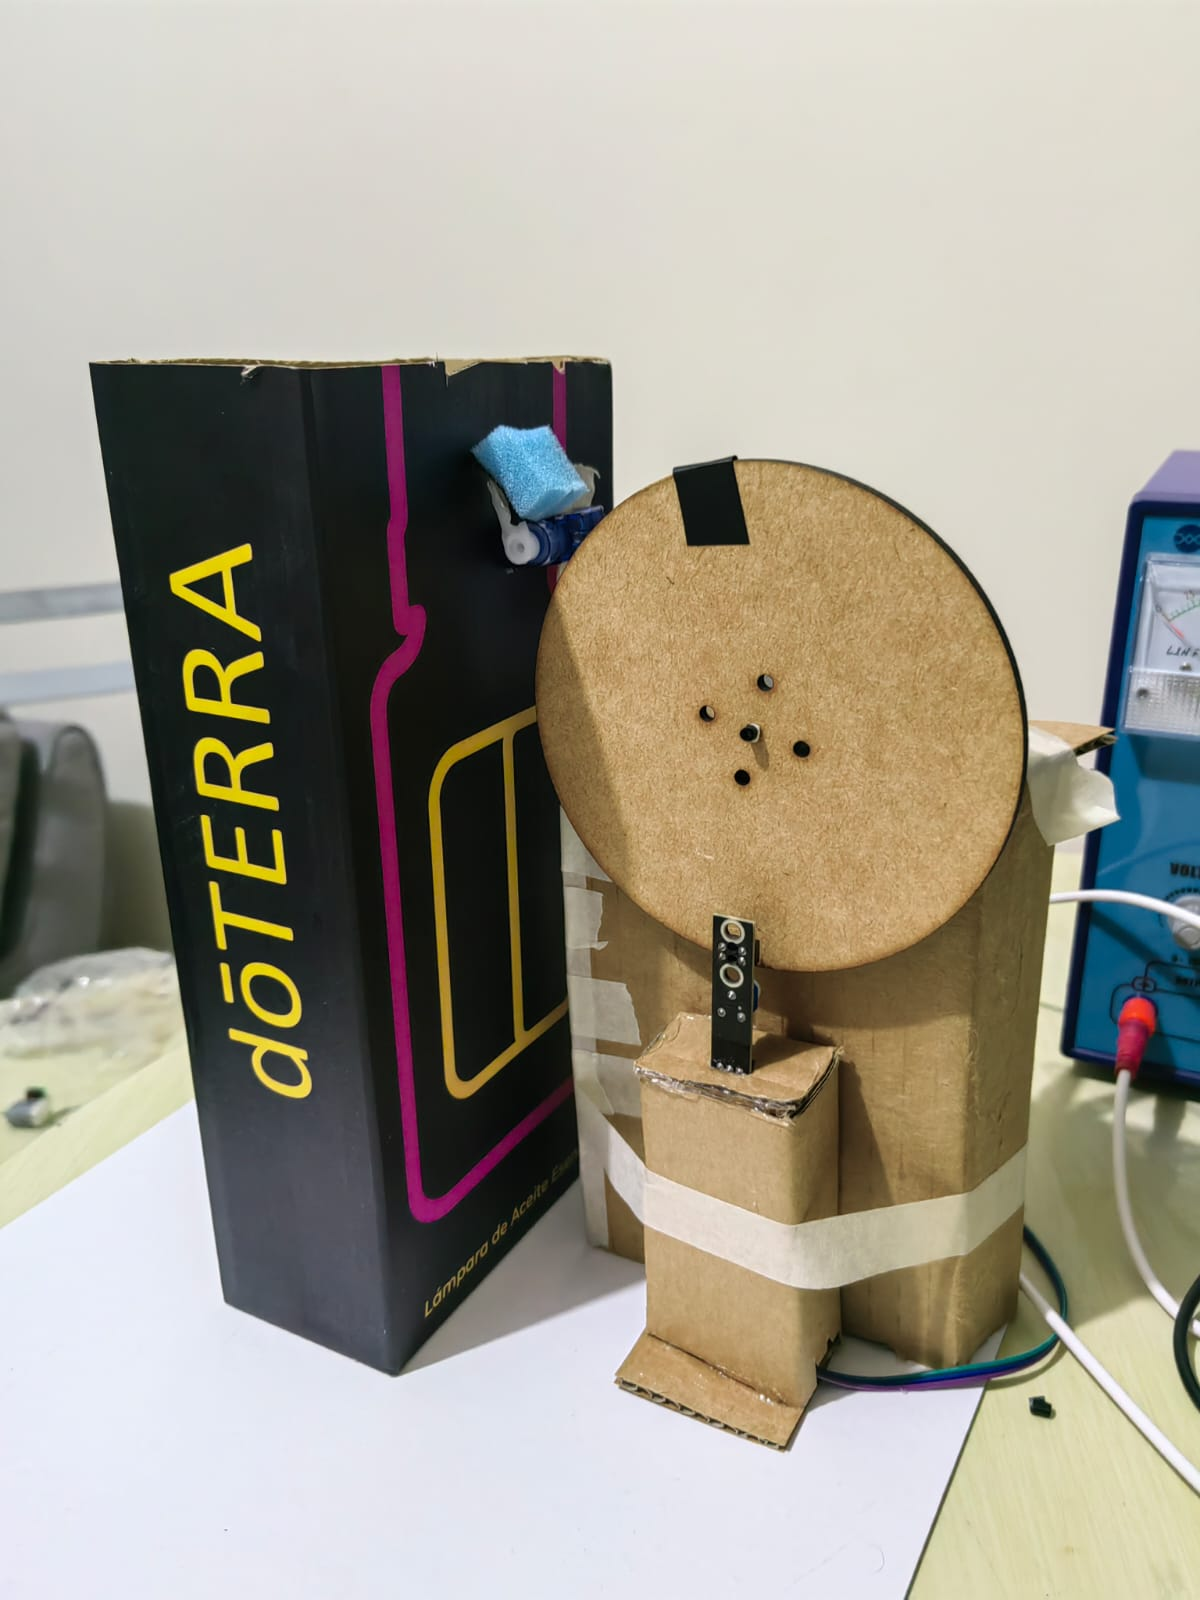
\includegraphics[width=\linewidth,height=0.32\textheight,keepaspectratio]{foto_montaje_general.jpeg}\\
\footnotesize (d) Vista general del banco y ubicación del KY-033 bajo el disco.
\end{minipage}
\caption{Fotografías del montaje real. La fuente alimenta el motor;
la ESP32 registra los pulsos del sensor y ordena el servomotor.}
\label{fig:fotos_montaje}
\end{figure}

\begin{figure}[H]
\centering
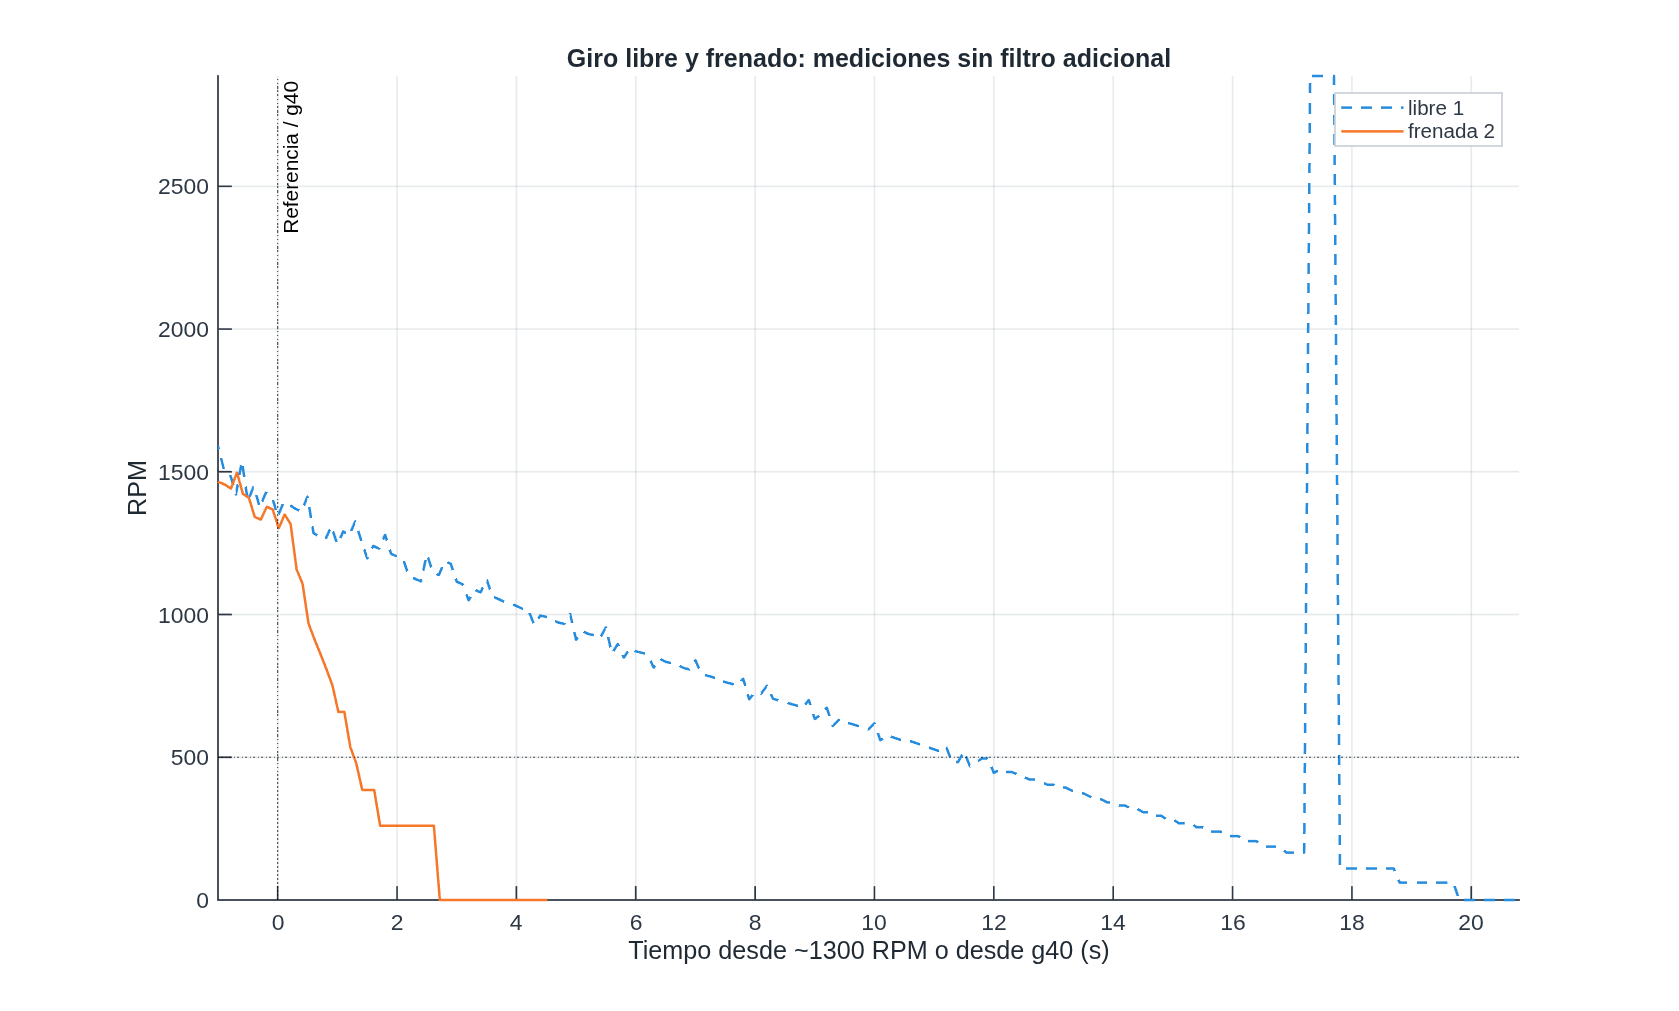
\includegraphics[width=0.85\textwidth]{comparacion_real.png}
\caption{Mediciones reales del giro libre (1) y frenado (2), alineadas
desde una velocidad cercana a 1300 RPM. La línea en $t=0$ es la
referencia de RPM para la libre y la orden \texttt{g40} para la frenada.}
\label{fig:comparacion_real}
\end{figure}

\begin{figure}[H]
\centering
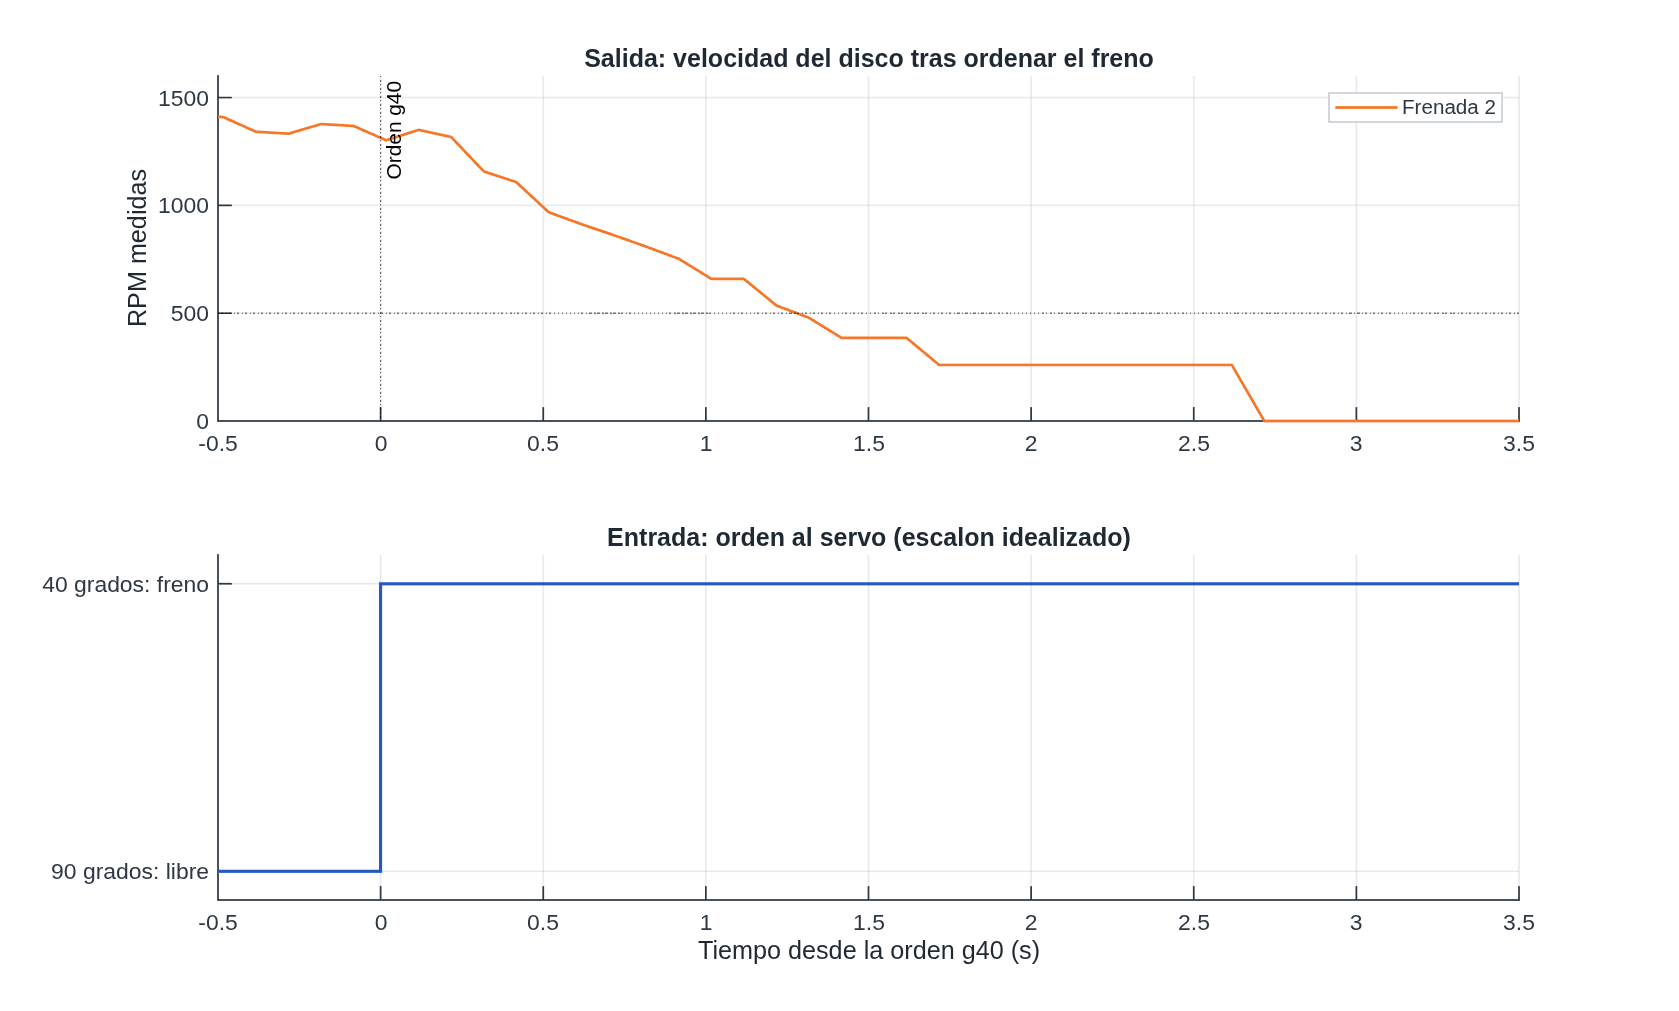
\includegraphics[width=0.85\textwidth]{respuesta_escalon_real.png}
\caption{Entrada de escalón ordenada al SG90 y salida de RPM medida
en la corrida frenada 2. El escalón corresponde al comando, no a un
cambio instantáneo verificado de fuerza de contacto.}
\label{fig:escalon_real}
\end{figure}

\begin{figure}[H]
\centering
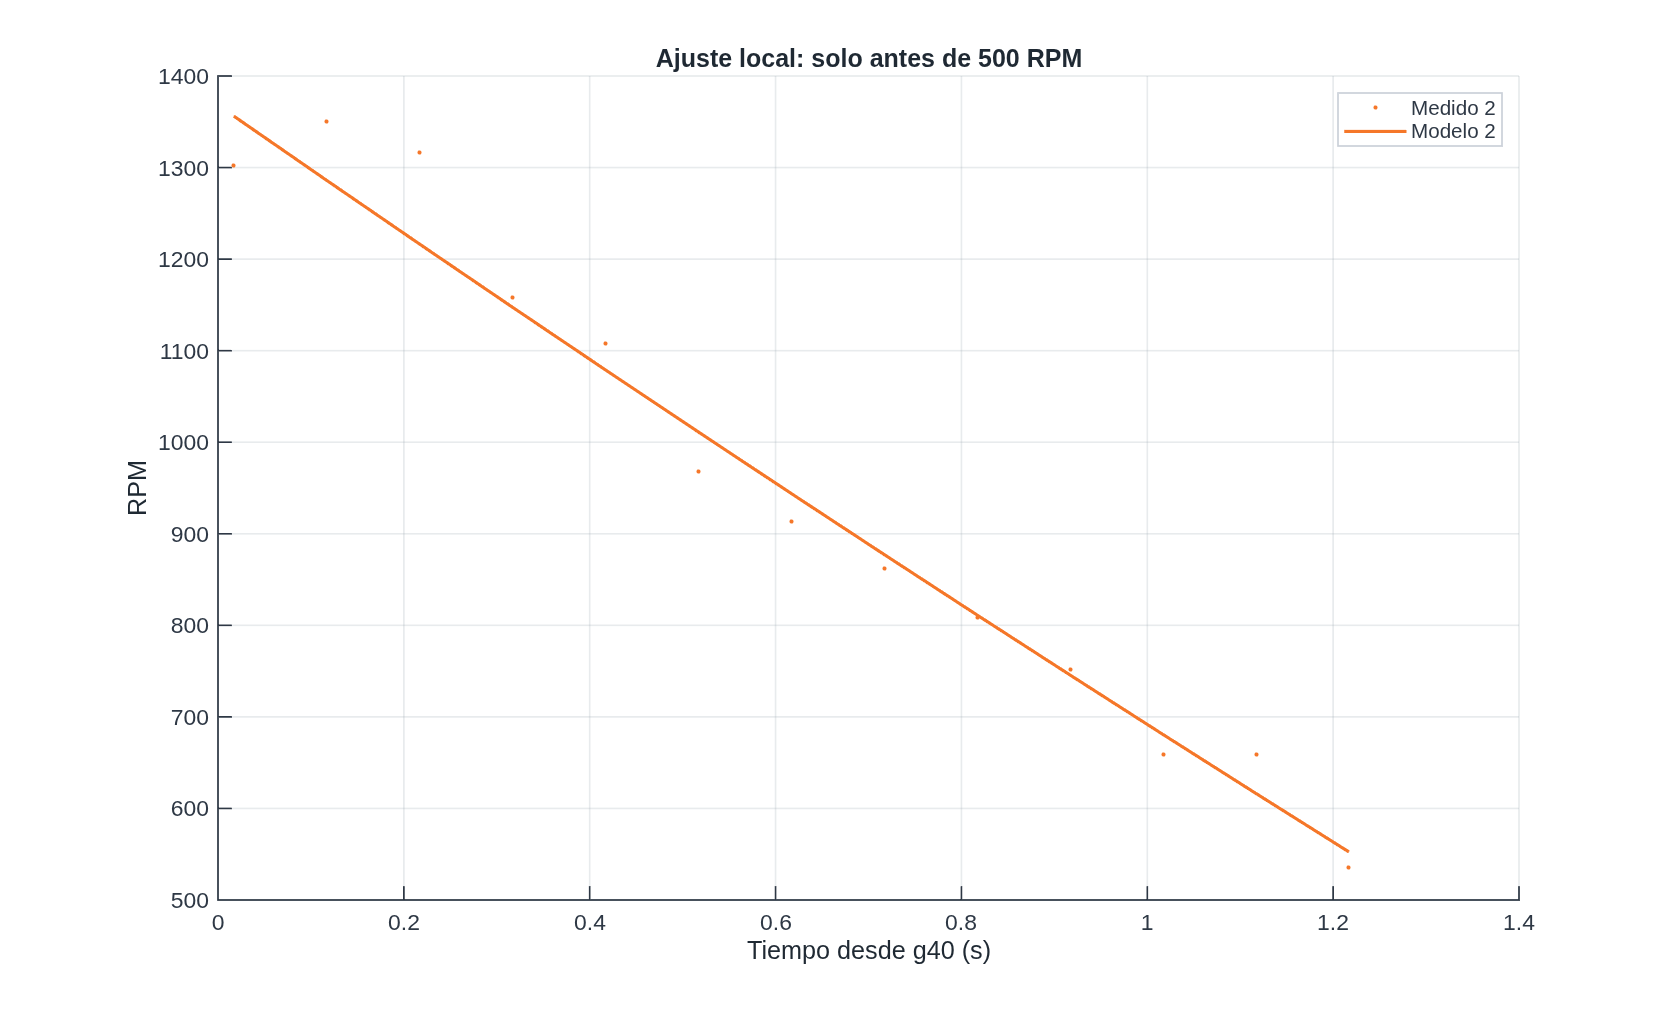
\includegraphics[width=0.85\textwidth]{ajuste_local.png}
\caption{Ajuste local de la frenada 2: muestras medidas y modelo
antes de bajar de 500 RPM. La extrapolación hasta cero no se valida.}
\label{fig:ajuste_local}
\end{figure}

\begin{figure}[H]
\centering
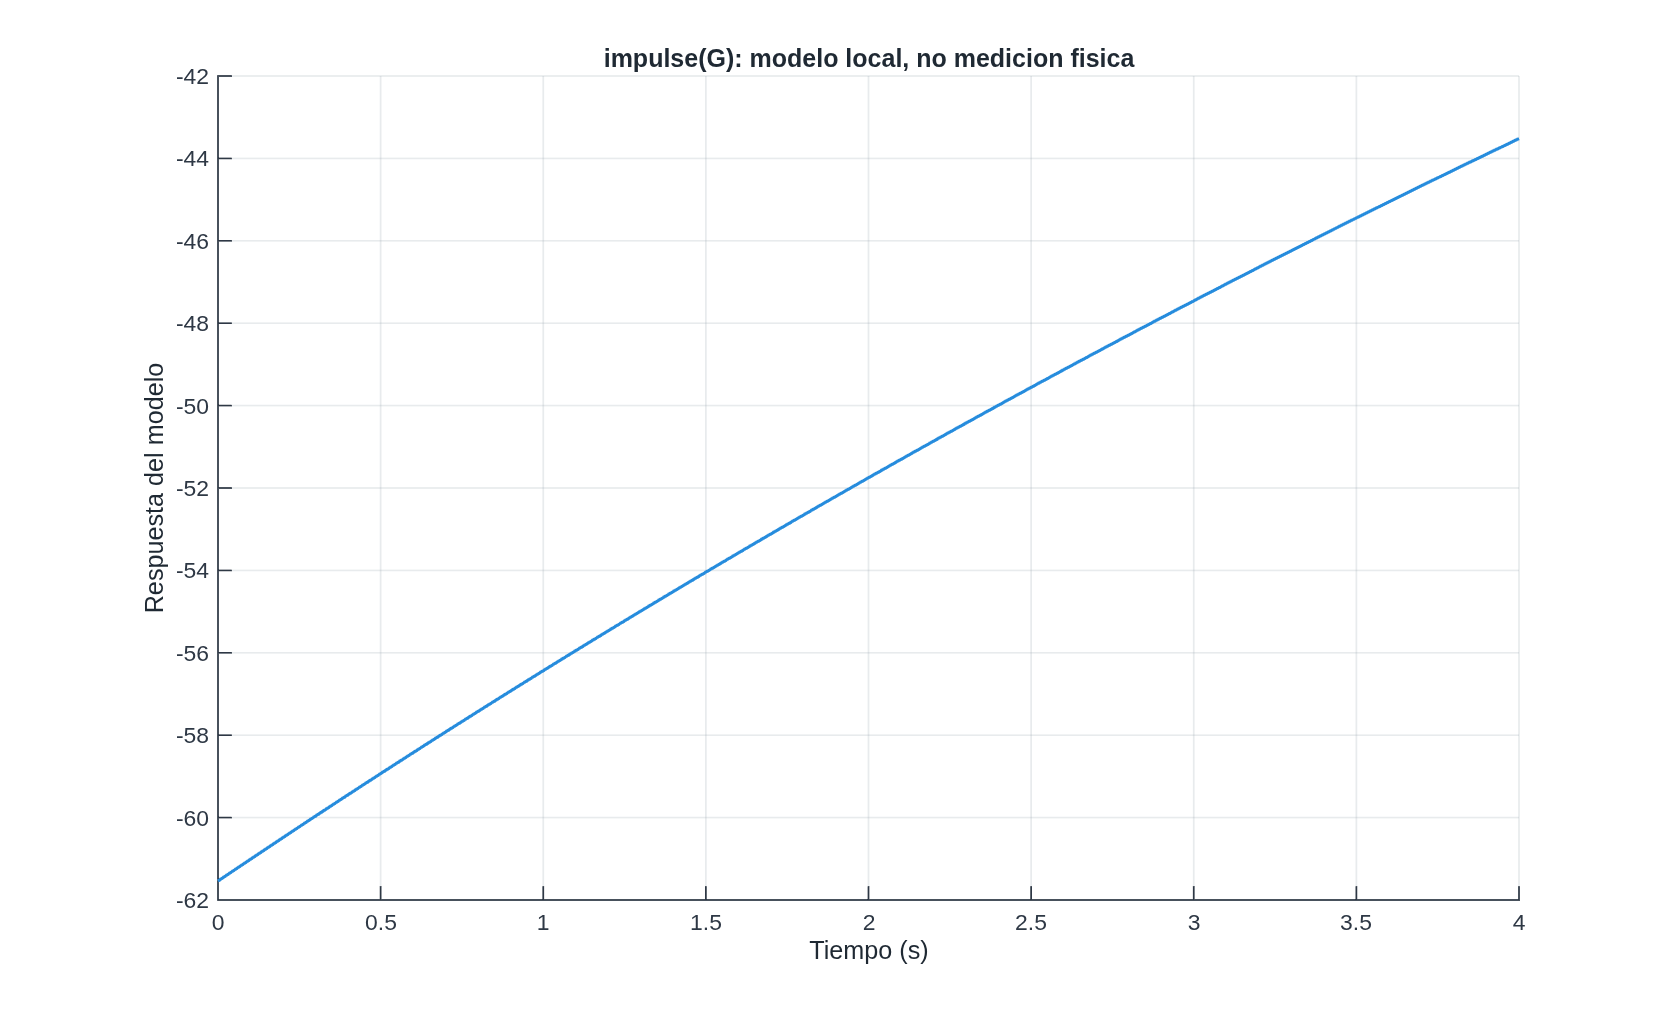
\includegraphics[width=0.85\textwidth]{impulse_matlab.png}
\caption{Respuesta impulsiva calculada por MATLAB para el modelo
local $G(s)$. Es negativa y tiende a cero desde abajo; se muestra
como resultado matemático del ajuste, no como prueba física.}
\label{fig:impulse_matlab}
\end{figure}

\end{document}
